\documentclass[12pt]{report}
\usepackage{vntex}
\usepackage{graphicx}
\usepackage{verbatim}
\usepackage[a4paper,width=150mm,top=25mm,bottom=25mm]{geometry}
\usepackage{listings}
\usepackage[
backend=bibtex,
style=numeric
]{biblatex}
\bibliography{thesis}

\title{Kỹ thuật dịch ngược}
\graphicspath{ {image/} }

\renewcommand*{\finalnamedelim}{\addcomma\addspace}
\begin{comment}
-	Lời cam đoan
-	Lời cảm ơn/ Lời ngỏ
-	Tóm tắt LV (bằng tiếng Việt và tiếng Anh)
-	Mục lục
-	Danh mục, bảng biểu, hình ảnh, ... (nếu có)
-	Nội dung LV (xem thêm phần Nội dung chi tiết ở Phần III)
-	Danh mục TL tham khảo
-	Phụ lục (nếu có)
\end{comment}
\begin{document}
	\pagenumbering{gobble}
	\chapter*{}
	\begin{center}
		ĐẠI HỌC QUỐC GIA TP. HCM\\
		TRƯỜNG ĐẠI HỌC BÁCH KHOA\\
		KHOA KHOA HỌC VÀ KỸ THUẬT MÁY TÍNH\\[10ex]
		\includegraphics[scale=0.5]{logoBK_jpg.jpg}\\[15ex]
		LUẬN VĂN TỐT NGHIỆP\\[10ex]
		\Large \textbf{KỸ THUẬT DỊCH NGƯỢC}\\[10ex]
	\end{center}
	
	
	\hspace*{7.5cm}GVHD: TS. Nguyễn Hứa Phùng\\
	\hspace*{8.15cm}GVPB: ThS. Võ Thanh Hùng\\[1ex]
	
	\hspace*{7.5cm}SVTH: Lâm Minh Phương - 51202846\\[8ex]
	
	\begin{center}
		\textit{Tp. Hồ Chí Minh, tháng 12/2016}
	\end{center}
	
	\chapter*{Lời cam đoan}
	\pagenumbering{Roman}
	
	Tôi xin cam đoan đây là công trình của tôi. Các số liệu, kết quả nêu trong báo cáo luận văn tốt nghiệp là trung thực và chưa từng được ai công bố trong bất kỳ công trình
	nào khác.\\
	Tôi xin cam đoan rằng mọi sự giúp đỡ cho việc thực hiện báo cáo luận văn tốt nghiệp này đã được cảm ơn và các thông tin trích dẫn trong báo cáo đã được ghi rõ nguồn gốc.
	
	\hspace*{8cm}\textbf{Sinh viên thực hiện}
	\\[10ex]
	\hspace*{9cm}Lâm Minh Phương
		
	\chapter*{Lời cảm ơn}
	Tôi xin gửi lời cảm ơn đến Tiến sĩ Nguyễn Hứa Phùng - Giảng viên trường Đại học Bách Khoa - Đại học Quốc Gia TP. HCM - đã giúp đỡ tôi trong suốt quá trình thực hiện luận văn này.\\
	Tôi cũng xin chân thành cảm ơn Michael James Van Emmerik, Trent Waddington và các lập trình viên đã phát triển nên nền tảng Boomerang.\\
	Ngoài ra, luận văn tốt nghiệp này là một sản phẩm kế thừa từ luận văn tốt nghiệp đề tài "Kỹ thuật dịch ngược" của Nguyễn Tiến Thành và Nguyễn Đôn Bình. Xin ghi nhận đóng góp của hai anh.\\
	Cuối cùng, xin gửi lời cám ơn đến các tác giả của tài liệu được trích dẫn trong báo cáo này. \cite{boomeranghomepage}
	
	\newpage
	\chapter*{Tóm tắt luận văn}
	Kỹ thuật dịch ngược ngày nay đã được ứng dụng nhiều trong ngành công nghiệp phần mềm. Để xây dựng một trình dịch ngược thành công, cần phải giải quyết nhiều bài toán phức tạp, chủ yếu liên quan đến việc khôi phục những thông tin không được lưu trữ ở ngôn ngữ gốc nhưng cần thiết phải có ở ngôn ngữ đích. Một trong những thông tin quan trọng nhất cần khôi phục là kiểu dữ liệu, và đã có nhiều giải pháp cho vấn đề này với độ chính xác chấp nhận được. Tuy nhiên, có những kiến trúc máy có các tính chất đặc biệt và đòi hỏi phải tạo ra một cấu trúc dữ liệu cấp cao phù hợp để đảm bảo mã cấp cao giữ nguyên được những tính chấp đó, cụ thể là cấu trúc union, và bài toán này vẫn chưa được giải quyết thấu đáo. Mục tiêu của luận văn là nghiên cứu và đưa ra những giải pháp phù hợp cho bài toán tìm kiếm union này.
	
	
	\newpage
	\tableofcontents
	
	\newpage
	\listoffigures
	
	\newpage
	\lstlistoflistings
	
	\newpage
	\pagenumbering{arabic}
	\chapter{Giới thiệu}
\label{sec:gioithieu}


Chương này nhằm giới thiệu về bài toán sẽ được giải quyết trong luận văn và các khái niệm liên quan. Đầu chương sẽ trình bày về kỹ thuật dịch ngược, các ứng dụng của nó và những khó khăn trong quá trình dịch ngược. Phần tiếp theo nêu bài toán đặt ra và các thách thức khi giải quyết bài toán. Phần cuối cùng sẽ tóm tắt cấu trúc của luận văn.

\section{Kỹ thuật dịch ngược và ứng dụng}
Trong khi kỹ thuật dịch phổ biến hiện nay là dịch từ mã viết bằng ngôn ngữ cấp cao xuống mã ngôn ngữ cấp thấp hơn, kỹ thuật dịch ngược thực hiện dịch từ mã ngôn ngữ cấp thấp lên mã ngôn ngữ cấp cao hơn. Kỹ thuật dịch ngược được sử dụng rất nhiều để hỗ trợ trong quá trình phát triển phần mềm:

\begin{itemize}
	\item Vì một lý do nào đó, mã nguồn của một phần mềm bị mất đi. Để tiếp tục phát triển hoặc bảo trì phần mềm đó, cần phải khôi phục lại mã nguồn. Nếu viết lại một chương trình mới hoàn toàn từ các tài liệu sẵn có sẽ rất mất thời gian và không đảm bảo sẽ tương đương được phần mềm cũ. Vì vậy một giải pháp phổ biến hiện nay là dựa vào file thực thi dịch ngược lại và hiệu chỉnh để có được mã nguồn mới hoàn chỉnh.
	\item Các phần mềm độc hại như virus, malware thường sẽ bị giấu kín mã nguồn. Kỹ thuật dịch ngược giúp sinh ra mã nguồn của chúng, qua đó, việc tìm ra phương pháp giải trừ sẽ dễ dàng hơn.
	\item Một số chương trình được viết để chạy trên các chip đã lỗi thời, như chip 8051, sẽ ngừng sản xuất trong tương lai gần, cần phải được chuyển đổi để chạy được trên những chip hiện đại hơn đang được sản xuất. Một trong những giải pháp để giải quyết vấn đề này là dùng trình dịch ngược để chuyển chương trình viết trên chip lỗi thời sang ngôn ngữ cấp cao, sau đó dùng trình biên dịch để dịch thành mã của chip thay thế. Cấu trúc của hệ thống chuyển đổi này được trình bày ở hình \ref{fig:fig12}.
	
	\begin{figure}[h]
		\centering
		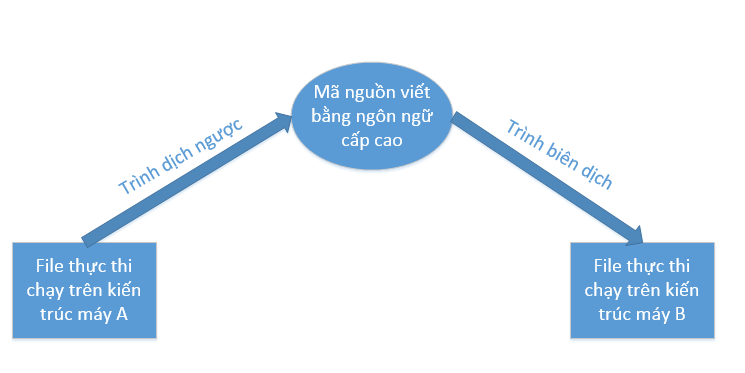
\includegraphics{fig12.png}
		\caption{Một ứng dụng của trình dịch ngược: chuyển đổi mã nguồn giữa các kiến trúc máy khác nhau}
		\label{fig:fig12}
	\end{figure}
	\item Phần mềm viết bằng ngôn ngữ A cần phải chuyển đổi sang ngôn ngữ B để tiếp tục bảo trì và phát triển. Ngôn ngữ A có thể là một ngôn ngữ đã ra đời từ rất lâu (ví dụ: COBOL, Basic...), hiện nay không còn người hiểu biết về ngôn ngữ đó để lập trình phần mềm. Vì vậy, cần phải chuyển đổi phần mềm sang một ngôn ngữ khác mới hơn, có nhân lực để phát triển tiếp (ví dụ: Java, C\#...). Quá trình này cũng được xem là dịch ngược, vì thường ngôn ngữ A ra đời trước sẽ có mức độ trừu tượng thấp hơn là các ngôn ngữ B được phát triển sau này.
\end{itemize}

Một trong những thách thức khó nhất của kỹ thuật dịch ngược là khôi phục thông tin. Do ở các ngôn ngữ cấp thấp không có phương tiện để lưu trữ một số thông tin cần thiết ở ngôn ngữ cấp cao, nên những thông tin đó sẽ bị mất đi trong quá trình dịch xuôi hoặc lập trình bằng ngôn ngữ cấp thấp. Một số thông tin cần khôi phục là:
\begin{itemize}
	\item Kiểu dữ liệu của biến: Đối với các chương trình viết bằng ngôn ngữ cấp cao, kiểu dữ liệu của biến có thể xem như một ràng buộc khi gán giá trị cho biến và sử dụng biến. Ví dụ khi ta khai báo một biến có kiểu dữ liệu là integer, thì ta phải gán cho biến các giá trị là số nguyên (1, 2,...) và sử dụng biến trong các phép toán nhận toán hạng là số nguyên. Nếu ta gán cho biến một giá trị khác số nguyên (số thực, chuỗi, boolean...) hoặc sử dụng biến trong các phép toán không chấp nhận toán hạng là số nguyên thì trình biên dịch sẽ phát hiện lỗi ngay ở giai đoạn đầu. Tuy nhiên, đối với một số mã máy, kiểu dữ liệu không cần thiết và sẽ được loại bỏ trong quá trình biên dịch. Khi dịch ngược, nếu không khôi phục được kiểu dữ liệu thì sẽ không đủ thông tin để xây dựng mã đầu ra.
	
	\item Tên của biến: Ở ngôn ngữ cấp cao, tên biến mang ngữ nghĩa là công dụng của biến đó, và được dùng để truy xuất giá trị của biến. Còn ở ngôn ngữ cấp thấp, dữ liệu sẽ được lưu vào các thanh ghi có sẵn hoặc vùng nhớ được truy xuất bằng địa chỉ trực tiếp, vì vậy việc tên biến ở cấp độ này là không cần thiết và sẽ bị loại bỏ. Nếu trình dịch ngược không giữ được tên biến của chương trình gốc thì rất khó để phát triển và bảo trì. Giải pháp hiện nay của các trình dịch ngược là sinh ra tên biến tự động, sau đó dựa vào các tài liệu sẵn có để chỉnh sửa tên biến bằng tay ở chương trình đầu ra. \cite{ssavan}
	
	\item Phân biệt giữa dữ liệu và mã điều khiển: Đặc điểm của một số mã máy (trừ mã máy chạy trên máy ảo) là dữ liệu và các câu lệnh điều khiển có cùng một định dạng mã nhị phân và được lưu trong cùng một vùng nhớ. Vì vậy, khi dịch ngược từ mã máy lên cần phải phân biệt được phần nào của vùng nhớ là lưu các dữ liệu và phần nào là câu lệnh của chương trình.
\end{itemize}

Từ khái niệm của kỹ thuật dịch ngược, có thể thấy có nhiều mức độ dịch ngược, tương ứng với những bài toán khác nhau cần giải quyết. Dựa vào các ứng dụng, suy ra được đầu vào của một trình dịch ngược có thể là: mã nhị phân, mã assembly hoặc mã của một ngôn ngữ lập trình cấp cao khác cần chuyển đổi. Tùy vào mức độ trừu tượng của ngôn ngữ đầu vào, các thông tin cần khôi phục sẽ khác nhau. Với mã máy thì tất cả các thông tin nêu trên đều không còn. Với mã assembly, tên biến vẫn xuất hiện trong chương trình vì một số assembler cho phép có các câu lệnh khai báo biến ở mã assembly. Còn với mã ngôn ngữ cấp cao thì gần như tất cả thông tin đều có ở chương trình gốc, và vấn đề cần giải quyết là tìm ra các cấu trúc tương đương ở ngôn ngữ đích.

\section{Bài toán đặt ra}
\label{sec:problem}
\subsection{Giới thiệu vấn đề}
Như đã trình bày ở trên, kiểu dữ liệu là một thông tin quan trọng không xuất hiện ở mã cấp thấp nhưng cần phải có để xây dựng mã đầu ra của trình dịch ngược. Vì vậy, bài toán suy luận kiểu là một thách thức cấp bách cần phải giải quyết trong kỹ thuật dịch ngược. Hiện nay, có nhiều nghiên cứu về vấn đề này và đưa ra những giải pháp khác nhau. Tuy nhiên, hầu hết chỉ giải quyết được những kiểu dữ liệu đơn giản như số nguyên, số thực, pointer... Còn các kiểu dữ liệu phức tạp hơn như structure, union, class... vẫn chưa được giải quyết hoàn toàn \cite{ssavan}. Mục tiêu của luận văn là giải quyết vấn đề khôi phục kiểu dữ liệu union. \\

Vấn đề này được đặt ra là do ở một số kiến trúc máy, một đối tượng dữ liệu (thanh ghi hoặc vùng nhớ) có thể được truy xuất ở nhiều cấp độ. Nghĩa là có thể truy xuất toàn bộ đối tượng đó, cũng có thể truy xuất một phần nhỏ hơn của nó. Khi thay đổi một phần đối tượng dữ liệu, thì đồng thời giá trị của toàn bộ đối tượng cũng thay đổi theo và ngược lại, khi thay đổi giá trị đối tượng đó, thì một phần nào đó của nó cũng sẽ thay đổi giá trị. Trong hình \ref{fig:eax}, thanh ghi \textit{eax} có độ dài là \textbf{32 bit}, tuy nhiên, người lập trình có thể truy xuất \textbf{16 bit đầu} của thanh ghi này bằng thanh ghi \textit{ax}. Và tương tự, \textbf{8 bit đầu} và \textbf{8 bit cuối} của \textit{ax} được thể hiện bằng các thanh ghi \textit{ah} và \textit{al}. Như vậy, khi thay đổi giá trị của thanh ghi \textit{ax}, thì giá trị của thanh ghi \textit{eax} cũng sẽ thay đổi theo và ngược lại.\\
\begin{figure}[h]
	\centering
	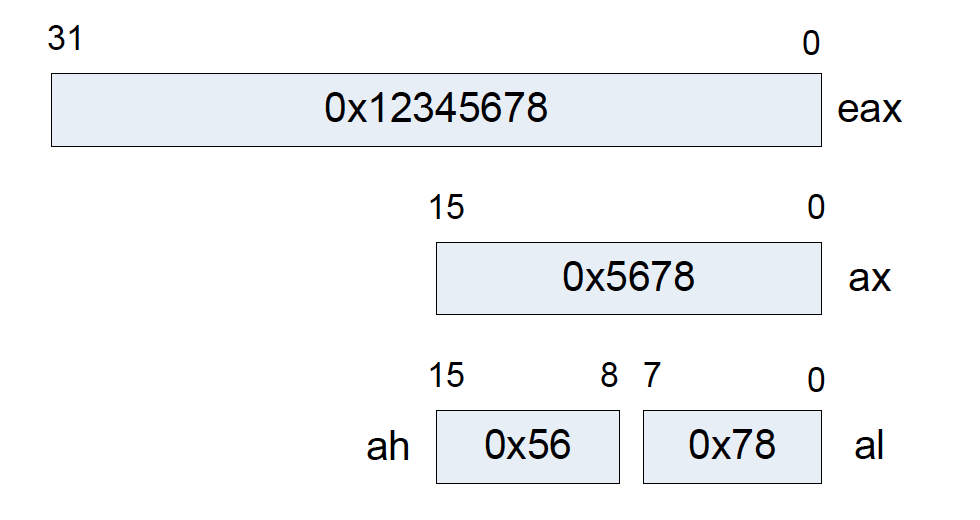
\includegraphics[width=0.7\linewidth]{image/eax}
	\caption{Thanh ghi eax trong kiến trúc máy x86}
	\label{fig:eax}
\end{figure}

Với tính chất trên, không thể xem phần nhỏ hơn của đối tượng dữ liệu (như thanh ghi \textit{ax}, \textit{ah}, \textit{al}) là những biến độc lập ở ngôn ngữ cấp cao, mà phải có cách nào đó thể hiện được mối quan hệ của chúng với toàn bộ đối tượng dữ liệu lớn (như thanh ghi \textit{eax}). Cấu trúc union ở ngôn ngữ cấp cao đáp ứng được yêu cầu đó. Vì cấu trúc union có tính chất là các thành phần cùng chia sẻ một vùng nhớ, nên khi thay đổi giá trị của một thành phần thì các thành phần còn lại cũng thay đổi theo, tương ứng với tính chất nêu trên ở mã assembly của một số kiến trúc máy. Như vậy, ta có thể xem toàn bộ đối tượng dữ liệu là một union với 2 thành phần:
\begin{itemize}
	\item Thành phần 1 cho phép truy xuất đến toàn bộ vùng nhớ.
	\item Thành phần 2 có kiểu dữ liệu là structure, cho phép truy xuất đến những phần nhỏ hơn của vùng nhớ đó.
\end{itemize}

Một trong những kiến trúc máy có những tính chất trên là 8051. Trong 8051, một số thanh ghi có thể được truy xuất ở mức bit, và đồng thời cũng có thể được truy xuất ở mức byte, ví dụ như thanh ghi \textit{ACC}. Như ví dụ trong hình \ref{list:8051exam1}, câu lệnh số 1 gán một giá trị cho thanh ghi \textit{ACC}, trong khi câu lệnh số 2 chỉ sử dụng bit đầu tiên của nó.

\begin{lstlisting}[caption={Đoạn mã 8051 sử dụng thanh ghi ACC ở nhiều cấp độ},label={list:8051exam1}]
MOV A, 38 ;1
SETB ACC.1 ;2
\end{lstlisting}

Ngoài ra, các vùng nhớ của 8051 cũng có tính chất tương tự. Trong ví dụ \ref{list:8051exam}, vùng nhớ có địa chỉ \textbf{38H} được load vào thanh ghi \textit{ACC} thông qua biến \textit{OPTIONS}, và biến \textit{TESTSUPS} đại diện cho bit đầu tiên của \textit{ACC} được sử dụng ngay sau đó. Từ đó, có thể kết luận \textit{ACC} chỉ là công cụ trung gian để thao tác trên vùng nhớ có địa chỉ \textit{OPTIONS} (sau này sẽ gọi tắt là vùng nhớ \textit{OPTIONS}), còn \textit{TESTSUPS} thực chất là bit đầu tiên của vùng nhớ đó. Như vậy, kiểu dữ liệu của vùng nhớ \textit{OPTIONS} là union và \textit{TESTSUPS} là một thành phần của union này.
\begin{lstlisting}[caption={Đoạn mã 8051 có một vùng nhớ mang kiểu union},label={list:8051exam}]
#DEFINE OPTIONS, #38H
#DEFINE TESTSUPS ACC.1
public AA
AA:
MOV A, OPTIONS ;1
SETB TESTSUPS ;2
\end{lstlisting}

\textit{Tóm lại, luận văn sẽ giải quyết vấn đề kiểm tra và suy diễn kiểu union từ mã assembly.} Đối với bài toán kiểm tra kiểu, người lập trình cần phải cung cấp thông tin về các kiểu union được sử dụng thông qua một phương thức nào đó. Chương trình sẽ khai thác thông tin đó và kiểm tra việc sử dụng kiểu union trong mã đầu vào có hợp lý hay không. Còn để suy diễn kiểu union, người lập trình không cần phải cung cấp thông tin, mà trình dịch ngược sẽ tự suy diễn ra các kiểu union thông qua quá trình phân tích việc sử dụng dữ liệu trong chương trình đầu vào. Các giải pháp này được trình bày trong sơ đồ khối \ref{fig:main}.

\begin{figure}
	\centering
	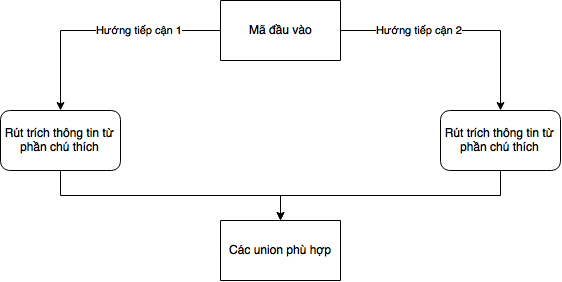
\includegraphics[scale=0.8]{image/main}
	\caption{Cách giải quyết các bài toán được trình bày trong luận văn}
	\label{fig:main}
\end{figure}

\subsection{Giới hạn bài toán}

Trong một kiến trúc máy, có hai kiểu đối tượng được dùng để lưu trữ dữ liệu là thanh ghi và vùng nhớ, luận văn sẽ giải quyết vấn đề khôi phục kiểu union của các vùng nhớ. Đối với các thanh ghi, mỗi kiến trúc máy đã có quy định sẵn thanh ghi nào có thể được truy xuất ở nhiều cấp độ. Một số thanh ghi ví dụ là \textit{eax} trong kiến trúc máy x86 và \textit{ACC} trong kiến trúc máy 8051. Như vậy, chỉ cần đọc đặc tả của kiến trúc máy là có thể biết được các thanh ghi nào có kiểu là union mà không cần phải phân tích gì thêm. Nhưng riêng với vùng nhớ, không có quy định nào đặt ra trước là những vùng nhớ nào được sử dụng như một union, những vùng nhớ nào không được sử dụng như vậy, nên cần trải qua một quá trình phân tích dữ liệu để xác định được kiểu dữ liệu của chúng. Vì vậy, các giải thuật trong luận văn này sẽ tập trung giải quyết vấn đề tìm kiếm kiểu union trên các vùng nhớ.\\

Ngoài ra, có rất nhiều kiến trúc máy có tồn tại kiểu union, nên luận văn sẽ chọn một kiến trúc máy để đưa ra các đoạn mã ví dụ và phân tích, cụ thể đó là 8051. Ngoài việc 8051 có các tính chất phù hợp với yêu cầu, một lý do nữa để chọn kiến trúc máy này là do nó đã lỗi thời và con chip 8051 sẽ bị dừng sản xuất trong tương lai gần, vì vậy, nhu cầu chuyển đổi mã từ 8051 sang một kiến trúc máy khác hiện đại hơn là có thật. Việc xây dựng giải thuật trên 8051 sẽ có thể ứng dụng ngay vào trình dịch ngược cho hệ thống chuyển đổi đó, giúp đưa ra kết quả chính xác hơn. Tuy nhiên, các giải thuật được nêu ra trong luận văn hoàn toàn có thể được áp dụng với những kiến trúc máy khác có tính chất tương tự 8051.

\subsection{Thách thức của bài toán}

Thách thức khó khăn nhất của bài toán là việc xác định các thành phần của một union đại diện cho vùng nhớ vì các thông tin ban đầu không đủ để kết luận điều đó. Như trong ví dụ \ref{list:8051exam}, thông tin ở phần khai báo ban đầu chỉ cho biết \textit{OPTIONS} mang giá trị là \textbf{38H}, và \textit{TESTSUPS} đại diện cho bit đầu tiên của thanh ghi \textit{ACC}, không có cơ sở nào để kết luận \textit{TESTSUPS} là một thành phần của union đại diện cho vùng nhớ \textit{OPTIONS}. Phải trải qua một quá trình phân tích dữ liệu, chỉ ra được rằng mỗi khi chương trình thao tác trên \textit{TESTSUPS}, thanh ghi \textit{ACC} luôn được load vào dữ liệu của vùng nhớ \textit{OPTIONS}, hay nói cách khác là thanh ghi ACC mang kiểu union \textit{OPTIONS}, thì mới xác định được \textit{TESTSUPS} là một thành phần thuộc union \textit{OPTIONS}. Như vậy, mấu chốt của bài toán là phải tìm ra được kiểu dữ liệu mà thanh ghi đóng vai trò trung gian đang mang và đây là một vấn đề phức tạp, đòi hỏi phải nghiên cứu nhiều phương pháp phân tích khác nhau để đưa ra được phương pháp có độ chính xác cao nhất và có thời gian xử lý chấp nhận được.


\section{Cấu trúc luận văn}

Luận văn gồm có 6 chương. Chương tiếp theo sẽ trình bày về các kiến thức nền tảng, cũng như một số nghiên cứu liên quan đến kỹ thuật dịch ngược. Ngoài ra, chương này cũng chỉ rõ kiến trúc của trình dịch ngược Boomerang và phần mở rộng của nó, nền tảng được dùng để hiện thực các nghiên cứu của luận văn. Chương 3 nêu ra giải pháp cho bài toán Kiểm tra kiểu. Tiếp theo đó, chương 4 trình bày cách giải quyết bài toán tiếp theo là Suy luận kiểu. Chương 5 giới thiệu một số thiết lập cần thiết trên trình dịch ngược Boomerang để kiểm tra kết quả các giải pháp đã đề ra ở những chương, cách thiết lập các mẫu thử (testcase) và kết quả chạy thử. Chương 6 kết luận về kết quả đạt được của luận văn và đề ra các hướng nghiên cứu tiếp theo.
	
\begin{comment}
Như đã đề cập ở phần trên, mục tiêu của luận văn là nghiên cứu về trình dịch ngược từ mã assembly lên mã cấp cao, các bài toán cần phải giải quyết và hiện thực giải pháp. Vì mã assembly cho kiến trúc máy khác nhau có những đặc điểm khác nhau, và đi cùng với đó là những vấn đề khác nhau cần giải quyết, nên giới hạn của luận văn sẽ là trình dịch ngược từ mã assembly 8051. Việc chọn kiến trúc máy 8051 là do 2 nguyên nhân sau:
\begin{itemize}
	\item Chip 8051 đã xuất hiện trên thị trường từ lâu, hiện tại sắp không còn được sản xuất. Tuy nhiên, vẫn còn nhiều hệ thống được chạy trên đây và cần phải chuyển đổi chúng sang một kiến trúc máy khác hiện đại hơn. Như vậy, nhu cầu đặt ra là có thực.
	\item Chip 8051 có một số đặc điểm khác biệt so với các con chip khác trên thị trường. Vì vậy việc dịch ngược từ mã 8051 sẽ gặp nhiều khó khăn hơn, vấn đề phải giải quyết phức tạp hơn. 
\end{itemize}

Các đặc điểm khác biệt của 8051 gồm có:
\begin{itemize}
	\item Trong khi hầu hết các kiến trúc máy khác sử dụng kiểu dữ liệu byte là kiểu dữ liệu nhỏ nhất, thì 8051 cho phép lập trình viên truy xuất tới mức bit trong một số thanh ghi và kèm theo đó là các câu lệnh xử lý bit. Tuy nhiên, các thanh ghi này của 8051 cũng có thể được truy xuất ở mức byte bình thường. Xem ví dụ ở đoạn mã \ref{list:list1}, câu lệnh số 1 gán giá trị ở vùng nhớ có địa chỉ 38H cho toàn bộ thanh ghi ACC, trong khi câu lệnh số 2 chỉ sử dụng biến số 1 của thanh ghi ACC.
	\begin{lstlisting}[caption={Một đoạn mã 8051 sử dụng cả biến bit và biến byte của thanh ghi ACC},label={list:list1}]
	MOV ACC, 38H #1
	SETB ACC.1 #2
	\end{lstlisting}
	\item Một số assembler của 8051 cho phép sử dụng tên biến. Biến này dùng để lưu các giá trị hằng số, hằng số này thường là địa chỉ một vùng nhớ kích thước 1 byte (trong luận văn này sẽ gọi tắt là biến byte) hoặc đại diện cho bit của thanh ghi (gọi tắt là biến bit). Khi lập trình, người ta thường sử dụng biến byte và biến bit này theo bộ, nghĩa là chỉ khi thanh ghi được load vào giá trị vùng nhớ quy định bởi biến byte, thì các biến bit cùng bộ mới được sử dụng (xem ví dụ ở đoạn mã \ref{list:list2}) (từ nay, khi luận văn sử dụng từ "nguyên tắc sử dụng bộ biến", nghĩa là đang đề cập đến nguyên tắc này).
		\begin{lstlisting}[caption={Một đoạn mã 8051 tuân theo nguyên tắc sử dụng bộ biến},label={list:list2}]
	#DEFINE OPTIONS #38H
	#DEFINE TESTSUP ACC.1
	public AA
	AA: 
	MOV ACC, OPTIONS
	JB TESTSUP, BB
	\end{lstlisting}
\end{itemize}

Từ các đặc điểm trên, ta có thể thấy bài toán lớn nhất đặt ra trong luận văn này sẽ là tìm ra được mối liên hệ giữa biến byte và biến bit trong chương trình, lấy được các bộ biến byte và biến bit đúng. Có 2 cách để biết được điều này:
\begin{itemize}
	\item Đưa ra quy định về việc khai báo biến byte và biến bit. Hiện nay, ở phần khai báo, các lập trình viên có thể khai báo các biến theo thứ tự tuỳ ý, và cũng không có quy định nào bắt buộc họ phải có phần comment chỉ rõ các biến byte và biến bit nào là cùng một bộ. Ta có thể đưa ra các mẫu khai báo cho biến byte và biến bit để trình dịch ngược có thể biết được các bộ biến bằng cách đọc theo mẫu mà không cần phân tích gì thêm. Tuy nhiên, sau khi đã xác định được các bộ biến này, cần có thêm một bước kiểm tra mã chương trình để đảm bảo rằng nguyên tắc sử dụng biến byte và biến bit được tuân thủ. Vì vậy, ta sẽ gọi giải pháp này là Kiểm tra kiểu - Type checking. Giải pháp này có ưu điểm là đơn giản, dễ hiện thực nhưng gây bất tiện cho người dùng vì phải chuyển đổi bộ mã hiện tại về theo mẫu quy định.
	\item Dựa vào phân tích luồng dữ liệu của chương trình, tìm ra được địa chỉ vùng nhớ được load vào thanh ghi tại thời điểm sử dụng biến bit và từ đó suy ra biến byte cùng bộ với biến bit đó. Giải pháp này được đặt tên là Suy luận kiểu - Type inference. Với cách làm này, không cần phải thay đổi đoạn mã gốc. Tuy nhiên cách hiện thực sẽ phức tạp hơn nhiều vì có rất nhiều cách load dữ liệu vùng nhớ vào thanh ghi như: dùng trực tiếp hằng số, dùng trực tiếp biến byte, trung gian qua một thanh ghi khác, dùng một biểu thức toán học có 2 vế... (xem ví dụ ở đoạn mã \ref{list:list3})
		\begin{lstlisting}[caption={Ví dụ một số mẫu câu lệnh load vùng nhớ vào thanh ghi trong 8051},label={list:list1}]
	MOV ACC, 38H
	MOV ACC, OPTIONS
	MOV ACC, @DPTR
	MOV ACC, OPTIONS+1
	\end{lstlisting}
\end{itemize}

Cả hai giải pháp này đều được hiện thực trong từng giai đoạn của luận văn và sẽ được trình bày trong các chương tiếp theo.

Ngoài ra, một công việc khác cần phải làm đó là giữ nguyên tên biến trong quá trình dịch ngược. Hiện tại trình dịch ngược Boomerang chỉ cho phép ta định nghĩa trước một số thanh ghi trong một kiến trúc máy, và đoạn mã đầu vào chỉ được sử dụng các thanh ghi đó, nếu sử dụng một cái tên nằm ngoài danh sách thanh ghi thì sẽ báo lỗi. Vì vậy, ta sẽ phải điều chỉnh cơ chế này, cho phép việc sử dụng tên biến khác và giữ nguyên chúng khi dịch ra đoạn mã ngôn ngữ cấp cao.

\section{Cấu trúc luận văn}
Luận văn sẽ gồm 6 chương như sau:
\begin{itemize}
	\item Chương 1: Giới thiệu về kỹ thuật dịch ngược, bài toán đặt ra trong luận văn và cấu trúc của luận văn.
	\item Chương 2: Nêu lên một số kiến thức cơ bản và các nghiên cứu liên quan đến luận văn. Đặc biệt, trong chương này sẽ trình bày một số kiến thức cơ bản về Boomerang, giúp người đọc dễ dàng hiểu các phần sau hơn.
	\item Chương 3: Trình bày giải pháp Kiểm tra kiểu - Type checking. Ngoài ra, trong chương này sẽ trình bày cơ chế cho phép đọc tên biến khác thanh ghi và lưu trữ chúng trong trình dịch ngược, vì đây là bước đầu tiên trong quá trình thực hiện các giải pháp.
	\item Chương 4: Trình bày giải pháp Suy luận kiểu - Type inference.
	\item Chương 5: Đánh giá kết quả của luận văn thông qua các mẫu thử (testcase).
	\item Chương 6: Kết luận.
\end{itemize}
\end{comment}
	\chapter{Các kiến thức nền tảng và nghiên cứu liên quan}
Chương này sẽ trình bày về một số kiến thức nền tảng như: trình biên dịch, trình dịch ngược, một số kỹ thuật thường được sử dụng trong trình dịch ngược và kiến trúc của trình dịch ngược Boomerang. Việc vì sao lựa chọn trình dịch ngược Boomerang để hiện thực các giải pháp cho bài toán cũng sẽ được bàn đến trong chương này. \\
\section{Trình biên dịch}
Trình biên dịch (compiler) là một chương trình hoặc một bộ chương trình máy tính, có nhiệm vụ biến đổi mã nguồn được viết bằng một ngôn ngữ lập trình này (ngôn ngữ lập trình gốc) sang một ngôn ngữ lập trình khác (ngôn ngữ lập trình đích), thường sẽ có dạng nhị phân và thực thi được. \\
Các bước của trình biên dịch gồm có:
\begin{itemize}
	\item Phân tích từ vựng (lexical analysis): Đây là quá trình chuyển hóa một chuỗi các ký tự (ví dụ như các câu lệnh trong một chương trình máy tính) thành chuỗi các từ tố (token), ví dụ như: định danh, số nguyên, số thực... Giai đoạn này kiểm tra các lỗi về từ vựng, chính tả của chương trình. \\
	
	Trong hình \ref{fig:lexi}, các ký tự \textit{a}, \textit{b} được nhận diện là các định danh (identifier), \textit{10} được nhận diện là số nguyên (integer), \textit{=} và \textit{+} được nhận diện là các phép tính (operator), \textit{;} là ký tự đặc biệt kết thúc một câu lệnh.
	
	\begin{figure}[h]
		\centering
		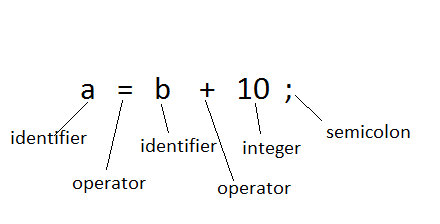
\includegraphics{fig21.png}
		\caption{Phân tích một câu lệnh thành các token}
		\label{fig:lexi}
	\end{figure}
	
	\item Phân tích cú pháp (syntax analysis): Từ chuỗi các từ tố được tạo ra ở giai đoạn trên, một chương trình gọi là parser sẽ tạo ra một cấu trúc dữ liệu, thường là parse tree hoặc abstract syntax tree. Giai đoạn này sẽ kiểm tra các lỗi về cấu trúc ngữ pháp.
	
	Câu lệnh gán từ ví dụ trên sẽ được phân tích thành cây cấu trúc như hình \ref{fig:parser}
	
	\begin{figure}[h]
		\centering
		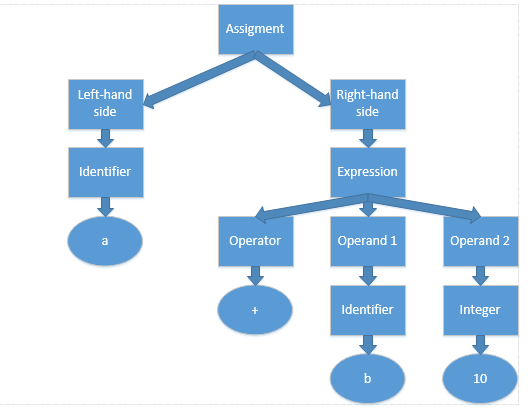
\includegraphics{fig22.png}
		\caption{Cây cấu trúc cho một câu lệnh gán}
		\label{fig:parser}
	\end{figure}
	
	\item Phân tích ngữ nghĩa (sematic analysis): Trong giai đoạn này, từ cây cấu trúc đã có, trình biên dịch sẽ áp dụng các luật về ngữ nghĩa để kiểm tra tính đúng đắn của chương trình. Thường sẽ là các luật về kiểu dữ liệu, kiểm tra tầm vực của biến và object binding.\\
	Tiếp tục ví dụ ở trên, trong gian đoạn này, trình biên dịch sẽ kiểm tra xem các biến \textit{a} và \textit{b} đã được khai báo chưa, tầm vực của các biến có phủ tới vị trí của câu lệnh không (ví dụ: có những biến được khai báo ở hàm \textit{A} thì sẽ không có tầm vực ở bên ngoài hàm \textit{A}), kiểu của biến có phù hợp với câu lệnh gán không (ví dụ: nếu \textit{b} có kiểu là \textbf{string} thì câu lệnh trên không hợp lệ).
	\begin{figure}[h]
		\centering
		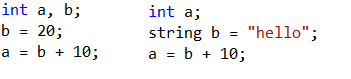
\includegraphics{fig23.png}
		\caption{Ví dụ về lỗi kiểu biến}
		\label{fig:semerror}
	\end{figure}
	
	Trong hình \ref{fig:semerror}, cả hai đoạn mã đều hợp lệ tính đến cuối giai đoạn phân tích cú pháp. Tuy nhiên, giai đoạn phân tích ngữ nghĩa sẽ phát hiện ra đoạn mã ở bên phải không hợp lệ vì nó vi phạm các ràng buộc về kiểu.
	
	\item Tạo ra mã trung gian: Sau khi trải qua các giai đoạn phân tích và kiểm tra, trình biên dịch sẽ tiến hành sinh mã trung gian từ mã nguồn. Đặc điểm của mã trung gian là đơn giản và rất gần với mã đích, tuy nhiên con người vẫn có thể đọc và hiểu được. Việc sinh mã trung gian nhằm giảm thiểu chi phí cho trình biên dịch khi phải sinh mã đích cho nhiều kiến trúc máy khác nhau. Thay vì với mỗi kiến trúc máy, trình biên dịch phải tạo ra công cụ riêng để dịch từ mã nguồn sang mã đích, thì ở đây chỉ cần tạo ra công cụ để dịch từ mã trung gian - vốn đã rất gần với mã đích.\\
	
	
	\item Tạo mã đích: Từ mã trung gian, tùy vào kiến trúc máy sẽ thực thi chương trình, trình biên dịch sẽ tạo ra mã đích tương ứng. Giai đoạn này sẽ thực hiện các công việc như: lựa chọn câu lệnh trung gian sẽ thực hiện, quyết định các giá trị được lưu trong thanh ghi, sắp xếp thứ tự thực hiện các câu lệnh. Đầu ra của giai đoạn là mã máy có thể thực thi được.
	
	
	\item Tối ưu mã đích: Để tăng tốc độ thực hiện chương trình cũng như giảm các chi phí chạy chương trình, giai đoạn tối ưu mã đích sẽ kiểm tra và áp dụng các kỹ thuật nhằm loại bỏ mã chết, tối ưu vòng lặp, loại bỏ dư thừa... Giai đoạn này không nhất thiết chỉ thực hiện ở cuối quá trình biên dịch mà có thể nằm ở bất cứ đâu.
\end{itemize}

\section{Trình dịch ngược}
Mục tiêu của trình dịch ngược là chuyển đổi chương trình được viết bằng một ngôn ngữ cấp thấp (thường là mã máy) lên một ngôn ngữ cấp cao hơn (như C, C++...). Vì vậy, trình dịch ngược (decompiler) có thể xem như một quá trình đảo ngược của trình biên dịch (compiler). Chương trình đầu ra phải thực hiện được những chức năng tương đương như chương trình đầu vào. \\

\begin{figure}[h]
	\centering
	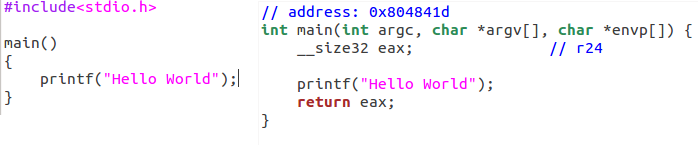
\includegraphics{fig24.png}
	\caption{Đoạn mã gốc và đoạn mã được dịch ngược bởi trình dịch ngược Boomerang}
\end{figure}

Qúa trình dịch ngược có thể chia thành các giai đoạn sau:
\begin{itemize}
	\item Loader: Load file cần dịch ngược, đọc từ file ra các thông tin như: loại file, loại kiến trúc máy... và xác định được ngõ vào của chương trình (tương đương với hàm main trong C).
	\item Disassembly: Mã gốc sẽ được chuyển thành mã trung gian, mã trung gian là gì thì tùy vào trình dịch ngược. Ví dụ Boomerang sẽ dùng mã trung gian là Register Transfer Language.
	\item Analysis: Sau khi đã chuyển sang mã trung gian, chương trình sẽ đi qua các bước phân tích để khôi phục lại thông tin đã mất trong quá trình biên dịch. Các phân tích thường phải có là: lan truyền biểu thức, loại bỏ mã chết, xác định nguyên mẫu hàm (function prototype), xác định kiểu dữ liệu...
	\item Code generation: Trải qua các kỹ thuật phân tích để xác định được thông tin cần thiết về dữ liệu, kiểu và luồng điều khiển chương trình, giai đoạn cuối cùng của dịch ngược là sinh ra mã chương trình bằng ngôn ngữ bậc cao. 
\end{itemize}
\begin{figure}[h]
	\centering
	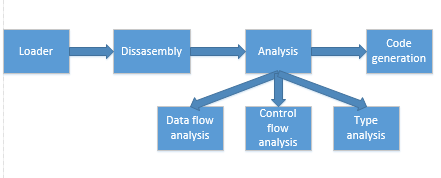
\includegraphics{fig27.png}
	\caption{Các bước cơ bản của một trình dịch ngược}
\end{figure}
\section{Một số kỹ thuật tiêu biểu được sử dụng trong các công cụ dịch ngược}
\subsection{Lan truyền biểu thức}
Lan truyền biểu thức (Expression propagation) là biến đổi phổ biến nhất trong quá trình dịch ngược một đoạn code. Nguyên tắc truyền biểu thức cũng rất đơn giản: Với các câu lệnh sử dụng giá trị của một biến nào đó, ta có thể thay tên biến đó bằng biểu thức nằm bên phải câu lệnh gán biến đó.\\
\begin{figure}[h]
	\centering
	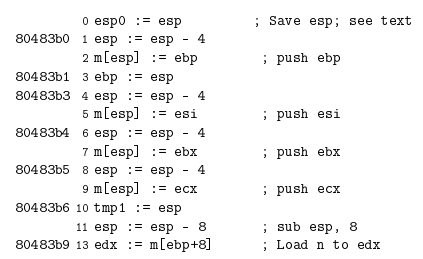
\includegraphics{fig33.png}
	\caption{Một đoạn mã trước khi thực hiện lan truyền biểu thức}
	\label{fig:33}
\end{figure}
\begin{figure}[h]
	\centering
	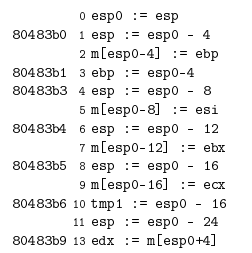
\includegraphics{fig34.png}
	\caption{Đoạn mã ở hình \ref{fig:33} sau khi thực hiện lan truyền biểu thức}
	\label{fig:34}
\end{figure}
Hình \ref{fig:33} và \ref{fig:34} là một ví dụ cho lan truyền biểu thức. Trong hình \ref{fig:33}, ta có các câu lệnh ở dạng mã trung gian trước khi thực hiện lan truyền biểu thức. Hình \ref{fig:34} là kết quả sau khi thực hiện lan truyền biểu thức. Ở đây ta giả sử có một biến đặc biệt là \textit{esp0} được gán giá trị là giá trị ban đầu của biến \textit{esp}. Ta sẽ thực hiện một thay thế đặc biệt ở câu lệnh số 1, thay vế phải của câu lệnh gán này - \textit{esp} - bằng biến tương đương với nó là \textit{esp0}. Sau đó, ở các câu lệnh tiếp theo, ta sẽ tiếp tục thay thế biến \textit{esp} bằng các biểu thức tương đương. Ví dụ: Ở câu lệnh số 2, biểu thức tương đương của \textit{esp} là \textit{esp0 - 4}, còn ở câu lệnh số 5, biểu thức tương đương của \textit{esp} là \textit{esp0 - 8} (do \textit{esp} đã được gán một giá trị mới ở câu lệnh số 4). Tuy nhiên, biểu thức \textit{esp0 - 8} không thể được dùng để thay thế cho biến \textit{esp} ở câu lệnh số 7 được, vì lúc đó \textit{esp} đã mang giá trị khác.\\

Như vậy, qua ví dụ trên, ta có thể thấy việc lan truyền biểu thức từ câu lệnh \textit{a} có dạng \textit{x := exp} đến một câu lệnh \textit{b} chỉ có thể được thực hiện nếu đáp ứng hai điều kiện sau:

\begin{itemize}
	\item \textit{a} phải là câu lệnh gán có vế trái là \textit{x} ở gần \textit{b} nhất. Nói cách khác, giữa \textit{a} và \textit{b} không được có bất cứ câu lệnh gán nào khác có vế trái là \textit{x}
	\item Trên tất cả các luồng đi của chương trình từ \textit{a} tới \textit{b}, không có câu lệnh gán nào có vế trái là bất kỳ biến nào được sử dụng trong \textit{a}
\end{itemize}
\begin{figure}[h]
	\centering
	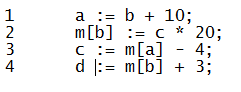
\includegraphics{fig35.png}
	\caption{Đoạn mã trung gian với bốn câu lệnh gán đơn giản}
	\label{fig:35}
\end{figure}
Ở đoạn code hình \ref{fig:35}, ta có thể thực hiện lan truyền biểu thức với biến \textit{a} ở câu lệnh số 3, kết quả sẽ là \textit{c := m[b + 10] - 4;} và câu lệnh gán biến \textit{a} sẽ được loại bỏ bằng kỹ thuật loại bỏ mã chết được bàn ở phần tiếp theo. Tuy nhiên, ta không thể thực hiện lan truyền biểu thức với \textit{m[b]} ở câu lệnh số 4, vì biến \textit{c} được sử dụng trong câu lệnh gán số 2 đã được sử dụng làm vế trái trong câu lệnh gán số 3.\\

Với mã trung gian như trên, để kiểm tra hai điều kiện thỏa mãn việc lan truyền biểu thức phải mất rất nhiều thời gian, ta phải xét hết tất cả các luồng chương trình từ câu lệnh gán đến câu lệnh sử dụng biến, kiểm tra tất cả các biến được sử dụng trong câu lệnh gán. Tuy nhiên, với mã SSA - sẽ được nói đến ở mục \ref{ssa}, hai điều kiện trên sẽ được tự động thỏa mãn và không cần bất kỳ kiểm tra gì thêm.
\subsection{Loại bỏ mã chết}

Mã chết bao gồm các câu lệnh gán mà biến ở vế trái của nó không bao giờ được dùng. Cần phân biệt mã chết (dead code) với mã không bao giờ được chạy (unreachable code), là những câu lệnh mà không có bất kỳ luồng điều khiểu hợp lệ nào của chương trình đi qua (ví dụ: câu lệnh ở dưới một vòng lặp vô hạn). Việc lan truyền biểu thức sẽ dẫn đến việc có một số biến không được sử dụng, từ đó sinh ra mã chết. \\
Từ đoạn mã đã được lan truyền biểu thức ở hình \ref{fig:34}, ta thấy biến \textit{esp} không được sử dụng ở bất kỳ câu lệnh nào. Vì vậy, các câu lệnh gán có \textit{esp} ở vế trái sẽ được xem là mã chết và được loại bỏ. Kết quả là hình \ref{fig:36}.

\begin{figure}[h]
	\centering
	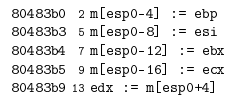
\includegraphics{fig36.png}
	\caption{Đoạn mã ở hình \ref{fig:35} sau khi loại bỏ mã chết}
	\label{fig:36}
\end{figure}

Để kiểm tra xem một biến có được sử dụng hay không, ta phải xem xét tất cả các luồng chạy hợp lệ của chương trình từ câu lệnh gán biến đến cuối chương trình, điều này phức tạp và mất nhiều thời gian. Tuy nhiên, mã SSA sẽ giúp việc kiểm tra mã chết dễ dàng hơn.
\subsection{Mã SSA} \label{ssa}

Mã SSA là một dạng mã trung gian có tính chất là: Mỗi biến hoặc vùng nhớ được định nghĩa duy nhất một lần trong toàn bộ chương trình. \\

Để chuyển từ mã RTL sang mã SSA, các biến cần phải được thay đổi tên, thường là sẽ được đánh số thứ tự đằng sau tên biến gốc. Ví dụ, nếu biến \textit{a} xuất hiện ở vế trái của 3 câu lệnh gán, thì sẽ được đánh số lần lượt là \textit{a1}, \textit{a2} và \textit{a3} như ví dụ ở hình \ref{fig:38}

\begin{figure}[h]
	\centering
	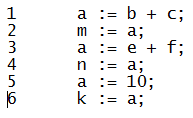
\includegraphics{fig37.png}
	\caption{Đoạn mã trung gian với 3 lần định nghĩa biến \textit{a}}
	\label{fig:37}
\end{figure}

\begin{figure}[h]
	\centering
	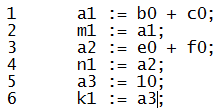
\includegraphics{fig38.png}
	\caption{Đoạn mã ở hình \ref{fig:38} đã được chuyển sang dạng mã SSA}
	\label{fig:38}
\end{figure}

Với tính chất của mã SSA, việc lan truyền biểu thức và loại bỏ mã chết sẽ được hiện thực rất dễ dàng.\\

Đối với lan truyền biểu thức, hai điều kiện đã được tự động thỏa mãn. Điều kiện đầu tiên thỏa mãn vì mỗi biến đều được định nghĩa duy nhất một lần, không có việc có nhiều định nghĩa cho cùng một tên biến (nếu ở mã gốc có việc đó, thì khi chuyển sang mã SSA, biến đó sẽ được đánh số để trở thành những biến khác nhau ở mỗi câu lệnh gán). Điều kiện thứ hai thỏa mãn vì chắc chắn từ câu lệnh gán một biến đến bất kỳ câu lệnh nào sử dụng biến đó, biến sẽ không được định nghĩa lại.\\

Việc loại bỏ mã chết cũng có thể thực hiện dễ dàng nhờ vào hành động thu thập thông tin về định nghĩa và sử dụng của một biến. Trong quá trình biến đổi từ mã RTL sang SSA, ta có thể xây dựng nên một bảng vị trí câu lệnh gán của một biến và vị trí các câu lệnh sử dụng biến đó. Trải qua các quá trình phân tích, nhất là lan truyền biểu thức, bảng này sẽ được cập nhật lại. Đến cuối cùng, các biến được định nghĩa nhưng không được sử dụng ở bất kỳ câu lệnh nào sẽ được xác định và loại bỏ các câu lệnh gán dư thừa đi.\\

\section{Tình hình phát triển trình dịch ngược hiện nay}
\label{sec:whyboom}
Hiện nay, có rất nhiều trình dịch ngược đã và đang được phát triển. Hầu hết đều hỗ trợ việc dịch ngược từ mã máy và có thể chia làm hai loại: trình dịch ngược nhận đầu vào là mã máy chạy trên máy ảo (ví dụ: mã máy được dịch từ các chương trình viết bằng Java, C\#) và trình dịch ngược nhận đầu vào là mã máy chạy trên máy thật. Loại thứ nhất có số lượng nhiều hơn, lý do có thể vì mã máy ảo còn lưu giữ được khá nhiều thông tin từ chương trình gốc, điển hình như tên biến toàn cục (xem hình \ref{fig:ilspy}). Vì vậy, bài toán cần giải quyết để xây dựng một trình dịch ngược dạng này không nhiều. Ngược lại, mã máy thật đã bị mất hầu hết các thông tin từ chương trình gốc, nên việc khôi phục thông tin ở các trình dịch ngược từ mã máy thật khá phức tạp. Trong hình \ref{fig:boomerang}, tên biến ở chương trình gốc đã bị mất đi. Ngoài ra, cấu trúc vòng lặp cũng thay đổi từ \textit{for} sang \textit{while}. Đó là do ở mã máy, cấu trúc vòng lặp ở ngôn ngữ cấp cao đã được dịch thành các câu lệnh kiểm tra điều kiện và jump, nên Boomerang phải sử dụng các thuật toán phân tích luồng điều khiển để tạo ra cấu trúc vòng lặp mới, đôi khi có thể không trùng khớp với cấu trúc vòng lặp ban đầu.

\begin{figure}[h]
	\centering
	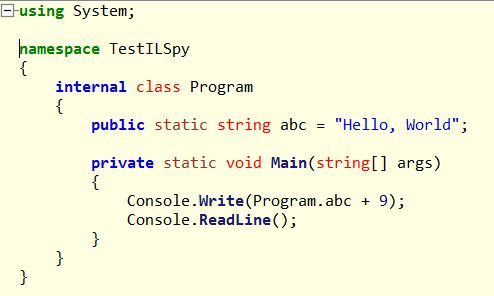
\includegraphics{fig25.png}
	\caption{Một đoạn mã được dịch ngược bởi trình dịch ngược ILSpy. Tên biến static \textit{abc} được giữ nguyên như mã gốc}
	\label{fig:ilspy}
\end{figure}
\begin{figure}[h]
	\centering
	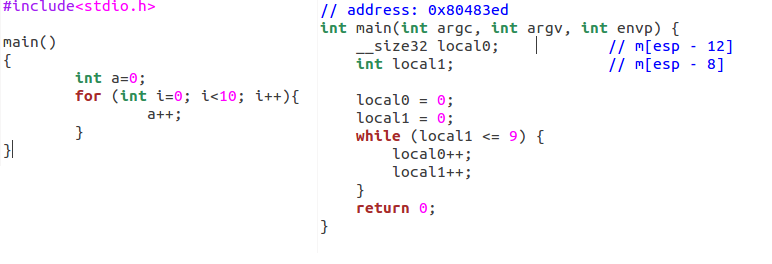
\includegraphics{fig26.png}
	\caption{Một đoạn mã được dịch bởi Boomerang}
	\label{fig:boomerang}
\end{figure}

Một số trình dịch ngược phổ biến có thể kể đến là:

\begin{itemize}
	\item dcc: Là một trình dịch ngược từ mã máy, đây được xem là một trong những trình dịch ngược đầu tiên và vẫn còn được phát triển tới bây giờ.
	\item ILSpy: Là một trình dịch ngược cho .NET, input là các file assembly được dịch từ chương trình .NET, được phát triển bởi isharpcode. Hiện nay ILSpy vẫn đang được tiếp tục phát triển và thêm các tính năng mới.
	\item Procyon: Là một trình dịch ngược cho Java. Trước đây lựa chọn hàng đầu để dịch ngược mã Java là JAD (Java decompiler), tuy nhiên hiện nay JAD đã ngừng phát triển và mã nguồn không còn mở nữa. Một số trình dịch ngược khác được phát triển và Procyon là một đại diện tiêu biểu.
	\item Boomerang: Là trình dịch ngược từ mã máy, mục tiêu là tạo ra một trình dịch ngược không quan tâm tới ngôn ngữ viết ra chương trình gốc. Boomerang đã ngừng phát triển từ năm 2006 do hai lập trình viên chính bắt đầu làm việc cho một công ty mà lĩnh vực nghiên cứu của họ trùng lặp với Boomerang.
\end{itemize}

Trong số các trình dịch ngược nêu trên, cần tìm ra trình dịch ngược phù hợp nhất để làm nền tảng cho việc hiện thực những giải pháp mà luận văn đề ra. Để tìm ra trình dịch ngược đó, phải có sự phân tích, đánh giá sự phù hợp của những trình dịch ngược thông qua một số tiêu chí. Phần đánh giá này được thể hiện ở bảng \ref{table:table1}
\begin{table}[h!]
	\centering
	\begin{tabular}{ |p{0.7cm}| p{2cm}| p{1.5cm}| p{1.5cm}| p{2cm}| p{1.5cm}| p{1.5cm}
			| p{1.5cm}| p{1.5cm}| p{1.5cm}| }
	\hline
		STT & Tên trình dịch ngược & Phù hợp với bài toán cần giải quyết & General compiler & Mã máy lưu trữ được nhiều thông tin gốc của chương trình & Có người hỗ trợ & Có tài liệu đầy đủ & Viết bằng ngôn ngữ quen thuộc & Tổng điểm\\
		\hline
		1 & Boomerang & 1 & 1 &0 & 5 & 2 & 0 & 9\\
	\hline
		2 & ILSpy & 0 & 0 & 2 & 0& 3 & 2 & 7\\
		\hline
		3 & dcc & 1 &1&0&0&0&0&2\\
		\hline
		4&Procyon&0&0&2&0&3&2&7\\
		\hline
	\end{tabular}
	\label{table:table1}
	\caption{Bảng đánh giá các trình dịch ngược}
\end{table}
\section{Kiến trúc của Boomerang}
Phần này sẽ giới thiệu về cấu trúc code của Boomerang, giúp ích cho việc trình bày các giải pháp của bài toán ở chương kế.

Về mặt tổng thể, Boomerang gồm có các phần sau:
\begin{figure}[h]
	\centering
	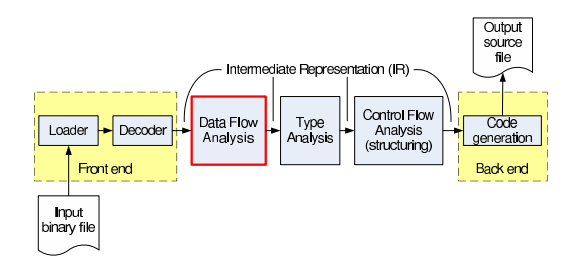
\includegraphics{fig32.png}
	\caption{Cấu trúc các khối lớn của Boomerang}
	\label{fig:boomstruct}
\end{figure}

Khi đọc vào một chương trình assembly, Boomerang sẽ lưu trữ chúng dưới cấu trúc được mô tả trong hình \ref{fig:assemblyinfo}.

\begin{figure}[h!]
	\centering
	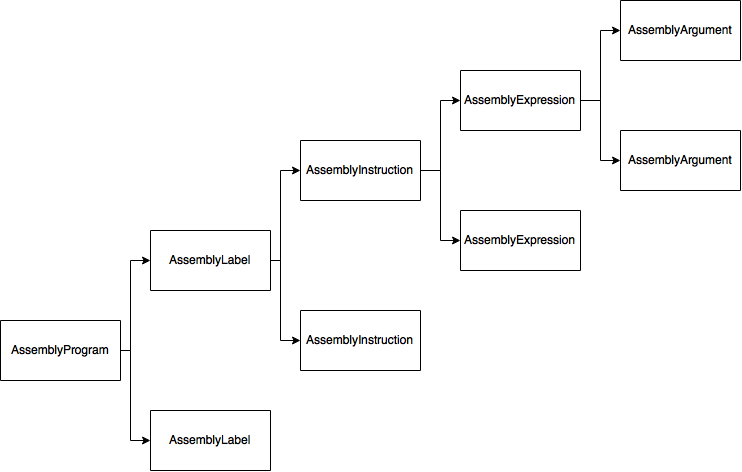
\includegraphics[width=0.7\linewidth]{assemblyInfo}
	\caption{Cấu trúc dữ liệu lưu trữ mã assembly trong Boomerang}
	\label{fig:assemblyinfo}
\end{figure}

Lưu ý, trong AssemblyArgument, giá trị thực sự của tham số được lưu vào một union có tên là Arg. Giá trị này có thể là một chuỗi (đối với trường hợp thanh ghi hoặc tên biến), một số nguyên, một số thực hoặc một structure đại diện cho bit (bao gồm tên thanh ghi và vị trí của bit). Đoạn mã \ref{list:assemblyinfo} thể hiện điều đó.
\begin{lstlisting}[caption={Đoạn mã mô tả cách biểu diễn giá trị của tham số trong Boomerang}, label={list:assemblyinfo}, language=c++]
struct bits{
	char* reg;
	int pos;
}
union Arg{
	int i;
	float f;
	char* c;
	bits bit;
}
\end{lstlisting}

Một lưu ý là cấu trúc nói trên chỉ áp dụng với các chương trình viết bằng ngôn ngữ assembly, còn khi viết bằng mã máy thì Boomerang sẽ sử dụng một cấu trúc khác, tuy nhiên, khi chuyển đổi chương trình đầu vào thành mã trung gian thì chỉ có duy nhất một loại cấu trúc cho tất cả các loại mã máy. Prog là tương ứng với toàn bộ chương trình. Một Proc là một hàm, BasicBlock đại diện cho một khối cơ bản mà ở đó không có một câu lệnh rẽ nhánh nào (ví dụ như if, hoặc vòng lặp...). Statement là một câu lệnh và Expr là các biểu thức trong chương trình. Ngoài ra còn có các class đại diện cho kiểu dữ liệu. Việc thực hiện các phân tích chủ yếu diễn ra tại Proc, vì vậy, các thay đổi trong luận văn này cũng chủ yếu được thực hiện bằng các hàm của Proc. Cấu trúc mã trung gian của Boomerang được thể hiện ở hình \ref{fig:progboomerang}\\
\begin{figure}
	\centering
	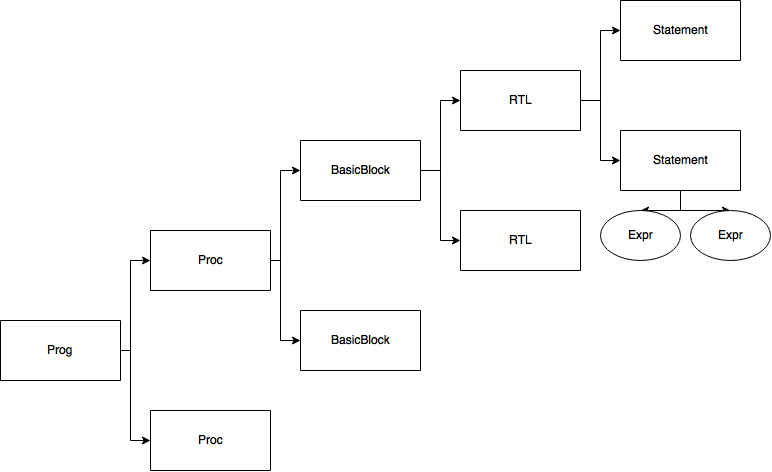
\includegraphics[width=0.7\linewidth]{progBoomerang}
	\caption{Cách lưu trữ một chương trình dưới dạng mã trung gian của Boomerang}
	\label{fig:progboomerang}
\end{figure}




Như vậy, để thực hiện việc xử lý mã 8051, ta cần phải chỉnh sửa các phần sau đây của Boomerang:
\begin{itemize}
	\item Phần parser để chấp nhận câu lệnh \#DEFINE, cũng như lưu trữ biến và giá trị của biến vào một bảng dữ liệu.
	\item Phần giải mã từ mã assembly lên mã trung gian để đưa các biến không phải thanh ghi thành một biểu thức trung gian phù hợp.
	\item Phần chuyển đổi từ biểu thức trung gian thành tên biến để giải quyết các trường hợp biến không phải thanh ghi. Hiện tại, Boomerang chỉ cho phép người dùng định nghĩa sẵn một danh sách thanh ghi của kiến trúc máy và dựa vào đó để chuyển đổi. Cần có cơ chế để Boomerang có thể chuyển đổi các biến ngoài danh sách thanh ghi đó.
	\item Phần phân tích dữ liệu của Boomerang để thêm vào một phân tích hỗ trợ cho việc nhận biết các bộ biến. Mỗi giải pháp sẽ có một phương pháp phân tích khác nhau và được trình bày ở các chương kế.
\end{itemize}
Các thay đổi này sẽ được trình bày kỹ hơn ở mục \ref{sec:boomchange}.
	\chapter{Kiểm tra kiểu - Type checking}
\label{chap:typechecking}
Chương này trình bày cách giải quyết bài toán Kiểm tra kiểu thông qua các bước sau:
\begin{itemize}
\item Mở rộng ngôn ngữ assembly để lưu trữ thông tin về kiểu union.
\item Kiểm tra tính hợp lệ của việc sử dụng kiểu union trong thân chương trình.
\end{itemize}
\begin{figure}[h!]
	\centering
	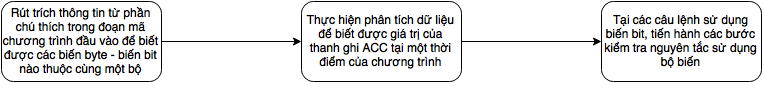
\includegraphics[width=\linewidth]{image/soDoTypeChecking}
	\caption{Sơ đồ các bước giải quyết bài toán Kiểm tra kiểu}
	\label{fig:sodotypechecking}
\end{figure}

Các phần tiếp theo của chương sẽ trình bày lần lượt các bước này.

\begin{comment}
\section{Chỉnh sửa để Boomerang chấp nhận việc sử dụng biến không phải thanh ghi}
\subsection{Cơ chế lưu trữ tên thanh ghi hiện nay của Boomerang}
Khi chuyển đổi từ mã assembly sang mã trung gian, Boomerang sẽ dùng một class con của Expr để biểu diễn thanh ghi. Cụ thể là class Location, và gọi phương thức static của class Location là Location::regOf(int num). Ta sẽ truyền vào phương thức này một con số đại diện cho thanh ghi đó. Cặp số - tên thanh ghi này được lưu vào một từ điển, để sau này khi thực hiện phân tích xong thì sẽ chuyển lại từ thanh ghi thành biến cục bộ.

Trong phần giải mã từ mã assembly sang mã trung gian, có một hàm để map giữa tên thanh ghi và con số đại diện cho nó, đó là hàm map\_sfr(string name).
\begin{lstlisting}[caption={Một số phần mã trong hàm map\_sfr},label={list:listmapsfr}]
if (name == "R0") return 0;
else if (name == "R1") return 1;
else if (name == "R2") return 2;
...
else return -1;

\end{lstlisting}

Sau khi trải qua các quá trình phân tích và đến giai đoạn in ra mã đầu ra, trình dịch ngược sẽ gọi hàm getRegName trong class FrontEnd để trả lại tên ban đầu của thanh ghi. Trong hàm getRegName sẽ lấy từ điển tên thanh ghi - số đại diện được quy định sẵn của mỗi phần giải mã cho các kiến trúc máy khác nhau, tìm tên thanh ghi tương ứng với con số đó và trả về.
\begin{lstlisting}[caption={Phần mã trong hàm getRegName},label={list:listgetregname}]
std::map<std::string, int, std::less<std::string> >::iterator it;
for (it = decoder->getRTLDict().RegMap.begin();	 it != decoder->getRTLDict().RegMap.end(); it++)
if ((*it).second == idx) 
return (*it).first.c_str();
return NULL;a
\end{lstlisting}


Như vậy, có thể thấy với các tên biến không được quy định trước, hàm map\_sfr sẽ trả về giá trị -1, và vì giá trị -1 sẽ không có trong từ điển của phần giải mã, nên hàm getRegName sẽ trả về NULL, dẫn đến trình dịch ngược sẽ bị lỗi runtime và dừng ngay lập tức.\\

%lấy mã Boomerang ban đầu về, hiện kết quả khi sử dụng biến đầu vào

Vì số lượng tên biến là rất nhiều, nên ta không thể sử dụng phương pháp thêm mới các tên biến vào từ điển được quy định sẵn được, mà phải có cách để trình dịch ngược linh động hơn, chấp nhận bất kỳ các tên nào được sử dụng trong mã assembly. Giải pháp đưa ra là ngoài việc sử dụng từ điển thanh ghi được quy định sẵn, ta sẽ lập thêm một bảng tên biến, thành phần bao gồm các cặp tên biến - số đại diện. Trong giai đoạn giải mã, khi hàm map\_sfr được gọi, nếu tên truyền vào nằm trong các thanh ghi đã quy định sẵn, thay vì trả về giá trị -1 thì ta sẽ tạo ra một giá trị random và đưa chúng vào bảng tên biến ở trên. Ngoài ra, còn có một đoạn mã kiểm tra biến được sử dụng đã được khai báo bằng câu lệnh \#DEFINE chưa (ngoại trừ một số biến đặc biệt được tự sinh). \\
\begin{lstlisting}[caption={Phần mã mới được bổ sung trong hàm map\_sfr},label={list:listmapsfrnew},language=c++]
bool isDefined = false;
map<char*, AssemblyArgument*>::iterator it;
for (it = replacement.begin(); it!=replacement.end(); it++){
if(strcmp((*it).first, name.c_str()) == 0 ){
isDefined = true;
break;
}
}
if (isDefined || name.find("specbits") != string::npos ){
if (symbolTable->find(name) == symbolTable->end()){
bool existed = false;
int num;
do{
num = std::rand()%200+31;
map<string, int>::iterator it;
for (it = symbolTable->begin(); it!=symbolTable->end(); it++){
bool cond1 = (*it).second == num;
bool cond2 = (byteVar != -1 && byteVar>=num);
bool cond3 = (bit != -1 && bit>=num);
if (cond1 || cond2 || cond3){
existed = true;
continue;
} else {
existed = false;
}
}
} while (existed); 
(*symbolTable)[name] = num;
if (name.find("specbits") != string::npos){
std::cout<<"Name: "<<name<<", "<<num<<endl;
}
return num;
} else {
return symbolTable->find(name)->second;
}
}
else {
std::cout<<"ERROR: "<<name<<" HAS NOT BEEN DEFINED YET"<<endl;
exit(1);
}
\end{lstlisting}
Tương ứng với sự thay đổi ở hàm map\_sfr,  ở hàm getRegName, ngoài việc dò trong từ điển quy định trước, ta sẽ thêm một đoạn mã để dò trong bảng tên biến. 
\begin{lstlisting}[caption={Phần mã mới được bổ sung trong hàm getRegName},label={list:listgetregnamenew},language=c++]
std::map<string,int>::iterator symIt;
for (symIt = decoder->getSymbolTable().begin(); symIt != decoder->getSymbolTable().end(); symIt++){
	if ((*symIt).second == idx){
		return (*symIt).first.c_str();
	}
}
\end{lstlisting}
Như vậy, vấn đề giữ nguyên tên biến được giải quyết mà không ảnh hưởng nhiều tới trình dịch ngược.
%đoạn mã đầu vào assembly và mã đầu ra giữ nguyên được tên biến
\end{comment}
\section{Mở rộng ngôn ngữ assembly}
Để kiểm tra được tính hợp lệ khi sử dụng kiểu union trong đoạn mã đầu vào, trình dịch ngược cần phải được cung cấp thông tin về các kiểu union thông qua một phương thức nào đó. Có hai hướng để giải quyết vấn đề này là:
\begin{itemize}
	\item Đưa ra một cấu trúc khai báo mới cho ngôn ngữ assembly. Cấu trúc khai báo này có thể tương tự như khai báo union ở ngôn ngữ cấp cao. Tuy nhiên, cách làm này sẽ làm cho đoạn mã assembly không thể compile được vì các assembler không chấp nhận cấu trúc mới thêm vào đó.
	\item Cho phép người lập trình đưa các thông tin về kiểu union vào trong phần chú thích theo một mẫu quy định từ trước. Với giải pháp này, đoạn mã không bị ảnh hưởng vì chú thích là một thành phần đã có sẵn trong ngôn ngữ assembly, và khi compile thì các assembler sẽ bỏ qua phần chú thích.
\end{itemize}
Như vậy, giải pháp thứ hai là tối ưu hơn và sẽ được áp dụng trong luận văn này. Mẫu chú thích được viết cho 8051 được thể hiện ở đoạn mã \ref{list:listdeclarevar}
\begin{lstlisting}[caption={Mẫu khai báo bộ biến},label={list:listdeclarevar}]
;BEGIN DEFINE
;DEFINE BYTE
[byte var declare]
;DEFINE BITS
[eight bit var declares]
;END DEFINE
\end{lstlisting}
Tuy nhiên, cũng giống như assembler, các trình dịch ngược hầu như sẽ bỏ qua phần chú thích khi đọc đoạn mã đầu vào, và để cho chúng có thể rút trích được thông tin từ phần chú thích thì phải thực hiện một số chỉnh sửa trong giai đoạn lexer và parser, cụ thể là:
\begin{itemize}
	\item Chỉnh sửa lexer để nhận biết các token là những chú thích đặc biệt. Như trong ví dụ \ref{list:listdeclarevar}, các chú thích ";BEGIN DEFINE", ";DEFINE BYTE", ";DEFINE BITS" không thể được đọc vào như là token COMMENT bình thường, mà phải có những token riêng biệt cho chúng để phục vụ giai đoạn parser sau đó. Đoạn mã \ref{list:8051lexer} được viết để chạy trên thư viện flex++ thể hiện điều đó. Có thể thấy, khi bắt được một chú thích, thay vì trả về token COMMENT như trước đó, phần lexer mới này sẽ kiểm tra nội dung chú thích, nếu trùng với các chú thích đặc biệt thì sẽ trả về token tương ứng. 
\end{itemize}
\begin{changemargin}{0cm}{0cm} 
	\begin{lstlisting}[caption={Phần lexer được chỉnh sửa để nhận biết các chú thích đặc biệt},label={list:8051lexer}]
	(\;.*)  { 
		string beginDefine = ";BEGIN DEFINE";
		string endDefine = ";END DEFINE";
		string defineByte = ";DEFINE BYTE";
		string defineBits = ";DEFINE BITS";
		string val = strdup(yytext);
		if (beginDefine == val)
			return BEGINDEFINE;
		else if (endDefine == val)
			return ENDDEFINE;
		else if (defineByte == val)
			return DEFINEBYTE;
		else if (defineBits == val)
			return DEFINEBITS;
		else return COMMENT;
		}
	\end{lstlisting}

\end{changemargin} 
\begin{itemize}
	\item Chỉnh sửa parser để nhận vào cấu trúc khai báo union. Tiếp tục với ví dụ mẫu khai báo \ref{list:listdeclarevar}, nếu phần parser chỉ đọc các câu lệnh khai báo biến bình thường, thì không thể xác định được các union mà người dùng khai báo trước. Như vậy, cần chỉnh sửa parser để bắt được những mẫu khai báo đặc biệt. Phần parser viết bằng thư viện bison++ cho mẫu khai báo \ref{list:listdeclarevar} được trình bày ở đoạn mã \ref{list:8051parser}. Trước khi chỉnh sửa, phần parser này chỉ có luật define, đọc vào từng câu lệnh khai báo độc lập. Sau khi được chỉnh sửa lại, luật definebit có độ ưu tiên cao hơn sẽ đọc vào cấu trúc khai báo union gồm nhiều câu lệnh khai báo khác nhau.
\end{itemize}
\begin{changemargin}{0cm}{0cm} 
	\begin{lstlisting}[caption={Đoạn mã parser nhận biết các mẫu khai báo union},label={list:8051parser}]
	definebit: BEGINDEFINE END_LINE DEFINEBYTE END_LINE 
					define DEFINEBITS END_LINE defineeachbit{8} 
					ENDDEFINE END_LINE;
	defineeachbit: DEFINE ID bit END_LINE;
	define:	DEFINE ID expressions END_LINE;
	\end{lstlisting}
\end{changemargin} 
\begin{itemize}
	\item Chỉnh sửa các hành động sau khi parser nhận biết được những cấu trúc khai báo union. Sau khi parser đã bắt được các mẫu khai báo union, cần lập trình để lưu trữ thông tin về các union đó vào dữ liệu của chương trình. Cấu trúc được dùng để lưu trữ thông tin về union này là UnionDefine, được trình bày ở đoạn mã \ref{list:listuniondefine}, trong đó, byteVar để lưu trữ tên của union đó, còn bitVar chứa các thành phần bit thuộc union và số thứ tự của bit mà thành phần đó truy xuất. Đoạn mã \ref{list:8051parser2} thể hiện phần code đưa các khai báo union từ mã đầu vào thành các thực thể UnionDefine tương ứng.
\end{itemize}
\begin{changemargin}{0cm}{0cm} 
	\begin{lstlisting}[caption={Cấu trúc dữ liệu để lưu trữ một union},label={list:listuniondefine},language=c++]
	class UnionDefine{
		public:
			char* byteVar;
			map<int, char*>* bitVar;
	};
	\end{lstlisting}
	\begin{lstlisting}[caption={Đoạn mã parser bao gồm các hành động sau khi nhận biết được union},label={list:8051parser2}]
	definebit: BEGINDEFINE END_LINE DEFINEBYTE END_LINE 
					define DEFINEBITS END_LINE defineeachbit{8} 
					ENDDEFINE END_LINE
	{
		UnionDefine* ut = new UnionDefine();
		$5 -> expList -> pop_back();
		ut->byteVar = $5 -> expList -> back() -> 
		argList.back()->value.c;
		ut->bitVar = bitVar;
		unionDefine1 -> push_back(ut);
		bitVar = new map<char*, int>();
	};
	defineeachbit: DEFINE ID bit END_LINE {
		std::string temp($3->value.c);
		char c =  temp.at(temp.size()-1);
		int num = c - '0';
		(*bitVar)[$2] = num;
	};
	define: DEFINE ID expressions END_LINE 
	{ 
		AssemblyLine* line = new AssemblyLine();
		line -> expList = new list<AssemblyExpression*>();
		line->kind = INSTRUCTION;
		line->name = "DEFINE";
		AssemblyExpression* expr1 = new AssemblyExpression();
		expr1 -> kind = UNARY;
		Arg a;
		a.c=$2;
		expr1 -> argList.push_back(new AssemblyArgument(6, a));
		line -> expList->push_back(expr1);
		line->expList ->push_back(expr);//*/
		expr = new AssemblyExpression();
		$$=line;
	};
	\end{lstlisting}
\end{changemargin} 
	
Như vậy, sau khi thực hiện các chỉnh sửa trên, trình dịch ngược đã có thể đọc vào các thông tin về union được người dùng cung cấp ở phần chú thích của đoạn mã đầu vào, đồng thời lưu trữ thông tin đó vào cấu trúc dữ liệu UnionDefine. Tuy đã xác định được những union nào được khai báo trong mã đầu vào, nhưng cần phải có một bước để kiểm tra những union đó có được sử dụng hợp lý hay không.
\section{Kiểm tra tính hợp lệ của việc sử dụng kiểu union}
Như đã trình bày ở phần \ref{sec:challenge}, ngôn ngữ assembly không cho phép thao tác trực tiếp trên các vùng nhớ, mà phải thông qua một thanh ghi trung gian và việc sử dụng một thành phần y thuộc union x chỉ hợp lệ khi mà thanh ghi trung gian đang mang kiểu union x đó. Như vậy, quá trình kiểm tra kiểu union sẽ gồm 2 bước:
\begin{itemize}
	\item Xác định kiểu của thanh ghi trung gian tại mỗi điểm của chương trình.
	\item Kiểm tra việc truy xuất thành phần của union có hợp lý hay không.
\end{itemize}
\subsection{Xác định giá trị kiểu của thanh ghi \textit{ACC} tại mỗi điểm của chương trình}
Để kiểm tra được nguyên tắc sử dụng bộ biến, trước hết, ta phải biết được tại mỗi thời điểm của chương trình, thanh ghi \textit{ACC} đang mang giá trị gì. Có hai phương pháp phân tích được áp dụng trong giải pháp này, đó là Reaching definitions kết hợp phần mở rộng và Type propagation.
\subsubsection{Phân tích Reaching definitions kết hợp phần mở rộng}
Mục đích của phân tích Reaching definitions là biết được ở một thời điểm của chương trình, các câu lệnh khai báo nào đang còn hiệu lực, hay nói cách khác là giá trị của các biến đang được khai báo bởi những câu lệnh nào. Phần mở rộng của Reaching definitions sẽ giúp xử lý thêm một số trường hợp, khi thanh ghi được truyền giá trị thông qua một thanh ghi trung gian khác.
\begin{figure}[h!]
	\centering
	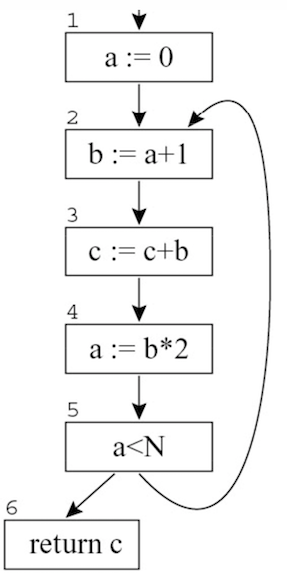
\includegraphics[scale=0.75]{image/reachingDefExam}
	\caption{Một đoạn chương trình mẫu}
	\label{fig:reachingdefexam}
\end{figure}
Ví dụ như ở đoạn chương trình \ref{fig:reachingdefexam}, cần biết được giá trị của biến \textit{a} ở câu lệnh số 2 được khai báo ở câu lệnh nào. Đối với con người thì rất dễ dàng biết được là biến \textit{a} được sử dụng có thể khai báo ở câu lệnh số 1 hoặc câu lệnh số 5. Tuy nhiên, cần có một phương pháp phân tích để cho máy tính cũng biết được điều đó, và đó chính là phương pháp Reaching definitions. Như vậy, khi áp dụng vào trình dịch ngược, ta sẽ biết được tại thời điểm sử dụng biến bit, giá trị của thanh ghi \textit{ACC} đang được định nghĩa ở câu lệnh nào. Từ đó tiến hành các bước kiểm tra tiếp theo. \\

Để thực hiện Reaching definitions, ta phải làm quen với các định nghĩa sau:
\begin{itemize}
	\item Nếu một biến được khai báo ở câu lệnh \textit{def1}, sau đó được khai báo lại ở câu lệnh \textit{def2} sau đó, thì ta nói là câu lệnh \textit{def1} đã \textbf{bị giết (killed)} bởi câu lệnh \textit{def2}.
	\item Nếu có một đường thực thi chương trình đi từ câu lệnh khai báo \textit{def1} đến một điểm \textit{p} của chương trình, mà trên đó \textit{def1} không bị giết bởi bất kỳ câu lệnh nào, thì ta nói là \textit{def1} đã \textbf{đến được (reach))} điểm \textit{p}. Khái niệm một câu lệnh đến được một khối cơ bản cũng tương tự như vậy.
\end{itemize}

Ngoài ra, ta phải quy định một số khái niệm mới cho một khối cơ bản B:
\begin{itemize}
	\item \textit{REACHin(B)}: Tập hợp các câu lệnh khai báo đến được đầu vào (entry) của B.
	\item \textit{REACHout(B)}: Tập hợp các câu lệnh khai báo đến được ngõ ra (exit) của B.
	\item \textit{GEN(B)}: Tập hợp các câu lệnh khai báo xuất hiện trong B và có thể đến được ngõ ra (exit) của B, nghĩa là biến được khai báo trong câu lệnh đó không được khai báo lại ở các câu lệnh đằng sau nó.
	\item \textit{KILL(B)}: Tập hợp các câu lệnh khai báo mà biến được khai báo đã được khai báo lại trong B.
\end{itemize}

Như vậy, mục tiêu của phân tích Reaching definitions ở cấp độ khối cơ bản là tìm ra được tập hợp \textit{REACHin} và \textit{REACHout} của từng khối. Công thức được áp dụng là;
\begin{equation} \label{eq:reachout}
	REACHout(B) = GEN(B) \cup (REACHin(B)-KILL(B))
\end{equation}	
\begin{equation} \label{eq:reachin}
REACHin(B) = \cup_{j \in Pred(B)} REACHout(j)
\end{equation}	

Từ hai công thức \ref{eq:reachout} và \ref{eq:reachin}, ta thấy ở phân tích này, tập hợp các giá trị ra (\textit{REACHin}) được quyết định bởi các giá trị vào (\textit{REACHout}), ngược lại với phân tích liveness (tìm tập hợp biến đang sống tại một thời điểm của chương trình). Như vậy, luồng đi của phân tích là cùng chiều với luồng đi của chương trình. Tương tự một số phương pháp phân tích dữ liệu khác, ta sẽ lần lượt tính toán các tập hợp vào và tập hợp ra của từng khối cơ bản cho đến khi không còn thay đổi nào được ghi nhận. Xem sơ đồ khối hình \ref{fig:reachingdefalgo}.



Tuy nhiên, trong trường hợp của bài toán cần giải quyết, ta cần phải biết tập hợp ra vào của từng câu lệnh một, chứ không chỉ của toàn bộ khối cơ bản, vì vậy, khi ứng dụng vào Boomerang, giải thuật sẽ được điều chỉnh lại để tìm tập \textit{REACHin} và \textit{REACHout} của từng câu lệnh. Việc điều chỉnh này là khá nhỏ, và các bước vẫn sẽ giữ nguyên, không thay đổi nhiều.\\

Khuyết điểm lớn nhất của phân tích Reaching definitions chỉ cho biết được câu lệnh khai báo có hiệu lực của một biến tại một thời điểm chương trình, chứ không cho biết được giá trị thực sự của biến đó. Cụ thể, với thanh ghi \textit{ACC}, nếu vế phải của câu lệnh khai báo này chỉ đơn giản là trỏ đến một vùng nhớ có địa chỉ được quy định bởi một biến byte thì biến byte đó sẽ được ghi nhận là đại diện cho vùng nhớ hiện thời \textit{ACC} đang lưu trữ. Nhưng ngoài ra, biểu thức quy định địa chỉ vùng nhớ được gán cho \textit{ACC} có thể là các trường hợp sau đây:
\begin{itemize}
	\item Một hằng số.
		\item Một thanh ghi, giá trị của thanh ghi có thể được khai báo ở các câu lệnh trước đó.
	\item Một biểu thức có hai vế, các vế của biểu thức có thể là một biến, một thanh ghi hoặc một hằng số.

\end{itemize}

\begin{lstlisting}[caption={Một số câu lệnh gán mà phương pháp Suy luận kiểu sử dụng Reaching definitions không xử lý được},label={list:listhardcase}]
MOV A, 38H #1
MOV A, @DPTR #2
MOV A, OPTION+1 #3
\end{lstlisting}
Các trường hợp phức tạp nêu trên được trình bày trong đoạn mã \ref{list:listhardcase}. 
Phương pháp Reaching definitions sẽ không thể xử lý được khi gặp các câu lệnh gán này. Ở câu lệnh số 1, phân tích có thể lấy được giá trị \textbf{38H}, nhưng không thể xác định được biến byte nào đã được khai báo giá trị \textbf{38H}. Ở câu lệnh số 2, Reaching definitions không thể biết được giá trị của thanh ghi \textit{DPTR} là bao nhiêu. Ở câu lệnh số 3, việc xử lý lại càng phức tạp hơn, vì nếu chỉ đơn giản lấy vế phải của khai báo ra, không thể nào biết được giá trị thực sự của nó là bao nhiêu.
Ngoài ra, với trường hợp trong tập hợp \textit{REACHin} của câu lệnh có nhiều câu lệnh khai báo cho thanh ghi \textit{ACC}, phương pháp này sẽ không thể kiểm tra được vế phải của tất cả các câu lệnh khai báo đó có cùng một giá trị hay không mà chỉ đơn giản xử lý là câu lệnh đã vi phạm nguyên tắc sử dụng bộ biến. Ví dụ như đoạn mã \ref{list:ifcond}, tại thời điểm câu lệnh sử dụng biến bit \textit{TESTSUPS}, có hai câu lệnh khai báo biến \textit{a} (là biến đại diện cho thanh ghi \textit{ACC} tại ngôn ngữ trung gian). Đối với phương pháp Reaching definitions, nó sẽ xem như có hai giá trị mà biến \textit{a} có thể mang, và sẽ báo lỗi vì vi phạm nguyên tắc sử dụng bộ biến. Tuy nhiên, nếu xét kỹ hơn, thì sẽ thấy là cả hai giá trị đó đều là biến \textit{OPTIONS}, và thực chất tại thời điểm này \textit{a} chỉ mang một giá trị, cho dù luồng đi của chương trình có như thế nào. Như vậy, phương pháp Reaching definitions sẽ bỏ qua những trường hợp như thế này và báo lỗi, dẫn đến việc độ chính xác sẽ không được cao.
\begin{lstlisting}[caption={Đoạn mã có nhiều câu lệnh khai báo cho ACC đến được một điểm của chương trình nhưng tất cả đều cùng giá trị},label={list:ifcond}]
if (...){
	a = *(OPTIONS);
	...
} else {
	a = *(OPTIONS);
	...
}
TESTSUPS = 1;
\end{lstlisting}

Để khắc phục phần nào khuyết điểm của Reaching definitions, một phần mở rộng được thêm vào để giải quyết một trong những trường hợp mà phương pháp này không thể giải quyết được. Đó là trường hợp sử dụng một biến trung gian và sử dụng hằng (câu lệnh số 1 và số 2 ở đoạn mã \ref{list:listhardcase}). Các trường hợp này được giải quyết nhờ vào việc lưu trữ các khai báo \textit{\#DEFINE} ở đoạn mã đầu vào, cũng như trong quá trình phân tích, tất cả các câu lệnh khai báo của tất cả các biến đến được một điểm trong chương trình đều được lưu giữ chứ không chỉ riêng của thanh ghi \textit{ACC}. Cụ thể các bước của phần mở rộng được trình bày ở hình \ref{fig:reachdefextendalgo}.
\begin{figure}
	\centering
	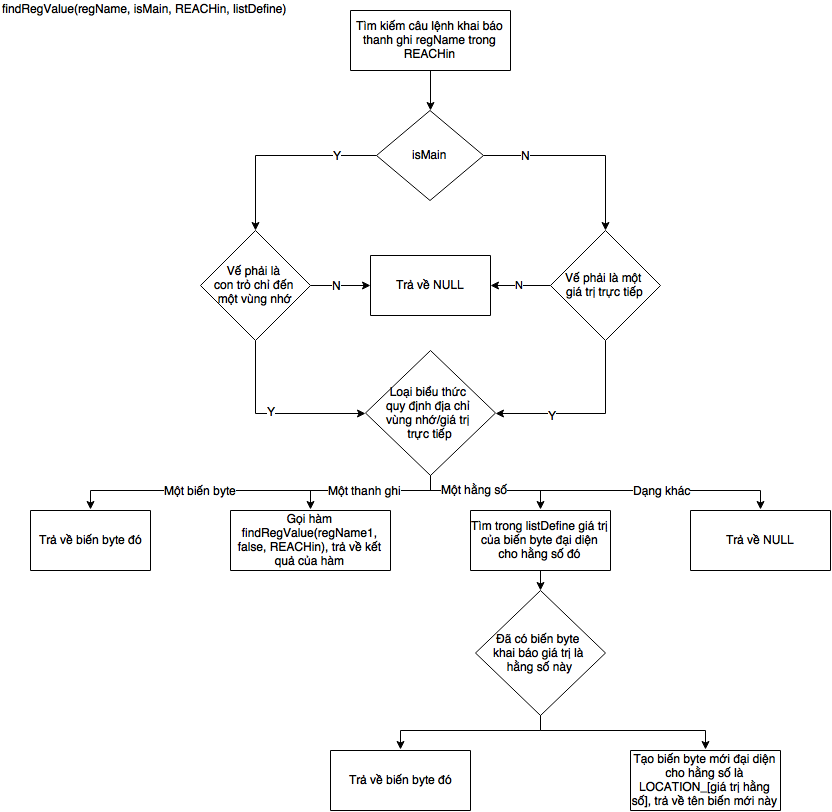
\includegraphics[width=0.7\linewidth]{image/reachdefextendalgo}
	\caption{Giải thuật cho hàm findRegValue - phần mở rộng của phân tích Reaching definitions}
	\label{fig:reachdefextendalgo}
\end{figure}

Theo giải thuật nêu trên, để tìm được giá trị của thanh ghi \textit{ACC} tại một thời điểm của chương trình, cần truyền vào hàm \textit{findRegValue} tên thanh ghi ("ACC"), giá trị true để hàm biết đang tìm kiếm giá trị cho thanh ghi \textit{ACC}, tập \textit{REACHin} tại thời điểm đó của chương trình và danh sách các cặp tên biến - giá trị biến được khai báo ở phần đầu của mã đầu vào. Qua các bước của giải thuật, hàm sẽ trả về giá trị là biến byte quy định vùng nhớ được load dữ liệu vào \textit{ACC} nếu tìm được biến này, còn nếu trả về giá trị \textbf{NULL}, nghĩa là giải thuật đã gặp phải trường hợp không xử lý được, đó là trường hợp biểu thức vế phải gồm hai toán hạng (câu lệnh số 3 của đoạn mã \ref{list:listhardcase}).

Tuy đã xử lý được hầu hết các trường hợp của phép gán cho \textit{ACC}, nhưng việc có thêm một phần mở rộng này sẽ làm cho tốc độ xử lý trình dịch ngược giảm đi. Cộng thêm việc bản thân giải thuật Reaching definitions đã có độ phức tạp cao, tổng thời gian xử lý cho bước này của trình dịch ngược là khá lớn. Vì vậy, một phương pháp phân tích khác đã được thực hiện để tìm ra giá trị của thanh ghi \textit{ACC} với độ phức tạp thấp hơn.

\subsubsection{Phân tích Type propagation}
Phân tích Type propagation có mục đích sẽ tìm ra được kiểu của một thanh ghi bằng cách lan truyền kiểu của những thanh ghi khác. Áp dụng vào trường hợp cụ thể của luận văn, các tên biến byte có thể được xem là một kiểu, vì khi chuyển đổi bộ biến thành một kiểu union ở ngôn ngữ cấp cao, tên biến byte này sẽ được dùng để đặt tên cho kiểu union đó. Như vậy, tác dụng của phân tích Type propagation này là tìm ra được thanh ghi \textit{ACC} đang mang kiểu union nào tại một thời điểm của chương trình. Các bước của giải thuật phân tích Type propagation được trình bày ở hình \ref{fig:typepropagationalgo}.

\begin{figure}[h!]
	\centering
	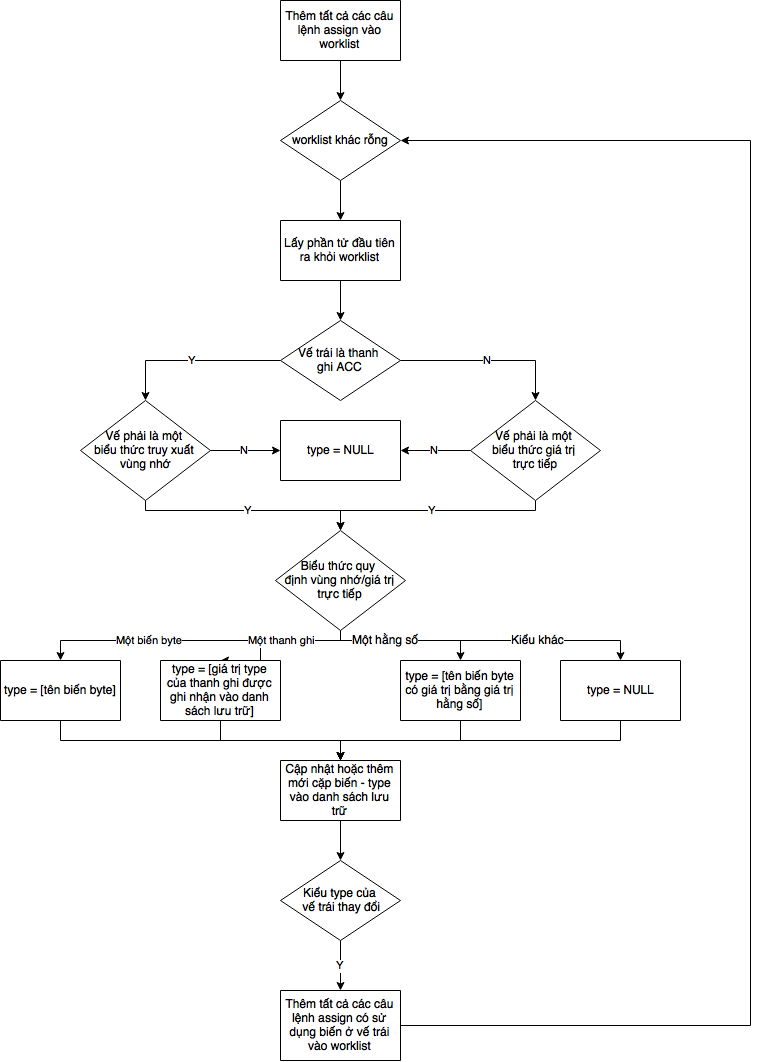
\includegraphics[width=0.7\linewidth]{image/typePropagationAlgo}
	\caption{Giải thuật của phân tích Type propagation}
	\label{fig:typepropagationalgo}
\end{figure}

Trong giải thuật đã trình bày ở trên, không xét đến trường hợp một biến được khai báo lại nhiều lần và tại mỗi thời điểm sẽ có giá trị khác nhau là do tận dụng được mã trung gian \textit{SSA}. Hầu hết các trình dịch ngược đều sử dụng mã \textit{SSA} tại một giai đoạn nào đó trong quá trình phân tích dữ liệu vì các lợi ích của loại mã này (chi tiết về mã \textit{SSA} được trình bày trong phần \ref{ssa}). Với mã \textit{SSA}, mỗi biến chỉ được khai báo một lần duy nhất trong chương trình, nên không bị ảnh hưởng bởi trường hợp khai báo lại biến.\\

Như vậy, phương pháp Type propagation này sẽ làm giảm đáng kể thời gian xử lý của chương trình so với phương pháp Reaching definitions. Khi có một thay đổi nào đó, chương trình phân tích chỉ cần tính toán lại các câu lệnh khai báo chịu ảnh hưởng của sự thay đổi đó, chứ không cần phải tính toán lại hết tất cả các câu lệnh như giải thuật của Reaching definitions. Phương pháp này cũng không cần một phần mở rộng mà ngay trong quá trình lan truyền, nó đã tính toán được các trường hợp biểu thức vế phải của khai báo là một thanh ghi hoặc một hằng số. Khuyết điểm của Type propagation là vẫn chưa xử lý được trường hợp biểu thức vế phải có hai toán hạng. Để giải quyết được vấn đề này, cần có một phân tích khác mạnh hơn và phân tích đó sẽ được giới thiệu ở chương tiếp theo.
\subsection{Kiểm tra tính hợp lệ về kiểu của tác vụ với bit}

\label{sec:laststep}

Sau khi đã tìm được thông tin về kiểu của thanh ghi \textit{ACC} tại mỗi điểm của chương trình, bước tiếp theo của giải pháp Kiểm tra kiểu là kiểm tra tính hợp lệ khi sử dụng các biến bit. Như đã trình bày ở phần \ref{sec:problem}, việc sử dụng các \textbf{biến byte - biến bit} trong mã chương trình 8051 cần tuân thủ các quy định sau:
\begin{itemize}
	\item Chỉ khi thanh ghi \textit{ACC} đang mang giá trị của vùng nhớ có địa chỉ quy định bởi biến byte, thì các biến bit cùng bộ mới được sử dụng.
	\item Mỗi biến bit chỉ thuộc một bộ duy nhất. 
	\item Tại mỗi vị trí bit của một bộ biến chỉ có một biến bit duy nhất tồn tại. 
\end{itemize}
Như vậy, ở phần này, chương trình sẽ chạy vòng lặp kiểm tra lần lượt từng câu lệnh sử dụng bit để xem xét việc sử dụng này có vi phạm quy định nào trong những quy định trên hay không. Các bước kiểm tra này được trình bày ở hình \ref{fig:checkunionsteps}.
\begin{figure}
	\centering
	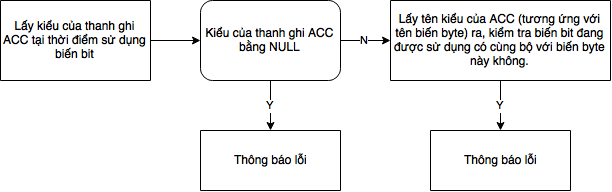
\includegraphics[width=0.7\linewidth]{image/checkUnionSteps}
	\caption{Quá trình kiểm tra một câu lệnh sử dụng bit}
	\label{fig:checkunionsteps}
\end{figure}
Nếu có một câu lệnh sử dụng bit nào đó vi phạm nguyên tắc trên, chương trình kiểm tra vẫn tiếp tục chạy để kiểm tra những câu lệnh sau đó. Điều này giúp người lập trình biết được tất cả các lỗi trong chương trình đầu vào của mình để có sự chỉnh sửa phù hợp. Tuy nhiên, khi có vi phạm xảy ra, trình dịch ngược sẽ không sinh được mã đầu ra, vì không có cách thể hiện union phù hợp.

%đoạn mã và output của trình dịch ngược khi vi phạm nguyên tắc sử dụng

Như vậy, với giải pháp Kiểm tra kiểu, ta đã có sẵn thông tin về bộ biến ngay từ đầu và chỉ cần kiểm tra xem người lập trình có tuân thủ đúng quy tắc không trước khi sinh ra mã ở ngôn ngữ cấp cao. Giải pháp này yêu cầu can thiệp vào trình dịch ngược ít và hiện thực dễ dàng. Tuy nhiên, giải pháp còn nhiều hạn chế như phương pháp phân tích dữ liệu chưa đạt độ chính xác cao, cần người dùng phải chỉnh sửa lại chú thích theo mẫu quy định... Chính vì vậy, giai đoạn sau của luận văn đã phát triển một hướng tiếp cận mới có độ chính xác cao hơn và không cần chỉnh sửa mã đầu vào của người dùng, đó là giải pháp Suy luận kiểu. Giải pháp này sẽ được trình bày ở chương tiếp theo.




	\chapter{Suy luận kiểu - Type inference}
Giải pháp Kiểm tra kiểu bắt buộc người lập trình chương trình đầu vào phải để lại chú thích ở phần khai báo biến, tuy nhiên, trong vì một số lý do, có thể phần chú thích này sẽ không xuất hiện hoặc không thể hiện đầy đủ thông tin, vì vậy cần có một giải pháp khác để xử lý trường hợp này. Giải pháp được giới thiệu ở chương này là Suy luận kiểu, với giải pháp này, bằng các phép phân tích dữ liệu, trình dịch ngược sẽ tự động tìm ra được các bộ biến được sử dụng trong chương trình. Các bước của giải pháp Suy luận kiểu gồm có:
\begin{enumerate}
	\item Xác định giá trị của thanh ghi ACC tại mỗi thời điểm của chương trình.
	\item Thông qua quá trình sử dụng biến của chương trình, lấy ra được mối quan hệ của các biến.
\end{enumerate}

\section{Xác định giá trị của thanh ghi ACC tại mỗi thời điểm của chương trình}
Tương tự như ở chương trước, bước đầu tiên của giải pháp Suy luận kiểu là xác định giá trị của thanh ghi ACC tại mỗi thời điểm của chương trình. Các giải pháp Reaching definitions mở rộng và Type propagation đã trình bày đều không thể xử lý hết tất cả các trường hợp xảy ra của phép gán thanh ghi ACC. Cụ thể, trường hợp không thể xử lý được là khi biểu thức quy định địa chỉ vùng nhớ của thanh ghi ACC là một biểu thức có hai toán hạng (xem ví dụ ở đoạn mã \ref{list:hardone}). 
\begin{lstlisting}[caption={Trường hợp không thể xử lý được bằng các phương pháp phân tích dữ liệu trước},label={list:hardone}]
MOV ACC, OPTIONS+1
\end{lstlisting}
Để mở rộng khả năng xử lý của trình dịch ngược, cần phải tìm ra một phương pháp khác tốt hơn. Phương pháp đạt yêu cầu phải tính toán được chính xác giá trị hiện có của thanh ghi ACC cho dù biểu thức bên phải của phép gán là gì. Cụ thể, chỉ các trường hợp giá trị ở thanh ghi ACC là một giá trị cố định, có thể tính toán được trước khi thực thi chương trình mới được xét đến vì nếu thanh ghi ACC có thể mang nhiều giá trị vùng nhớ khác nhau thì nguyên tắc sử dụng bộ biến sẽ bị vi phạm. Từ các yêu cầu trên, phương pháp phân tích phù hợp nhất trong trường hợp này là Lan truyền hằng số - Constant propagation. Phương pháp này cho phép tính toán giá trị của các biến, cho biết được giá trị đó có phải là một hằng số tại một thời điểm của chương trình hay không. Ví dụ như đoạn mã ban đầu \ref{list:listconstexam1}, chương trình phân tích có thể thấy giá trị của biến x là 14, nhưng không biết được giá trị thực sự của biến y, cũng như biểu thức trả về là bao nhiêu. Nhờ vào việc lan truyền hằng số, các giá trị này sẽ được tính toán, như trong đoạn mã \ref{list:listconstexam2} và \ref{list:listconstexam3}.
\begin{lstlisting}[caption={Đoạn mã trước khi thực hiện lan truyền hằng số},label={list:listconstexam1}, language=c++]
 int x = 14;
int y = 7 - x / 2;
return y * (28 / x + 2);
\end{lstlisting}
\begin{lstlisting}[caption={Đoạn mã sau khi thực hiện lan truyền hằng số cho biến y},label={list:listconstexam2}, language=c++]
int x = 14;
int y = 0;
return y * (28 / x + 2);
\end{lstlisting}
\begin{lstlisting}[caption={Đoạn mã sau khi thực hiện lan truyền hằng số cho biểu thức trả về},label={list:listconstexam3}, language=c++]
int x = 14;
int y = 0;
return 0;
\end{lstlisting}
Với phương pháp này, một biến có thể có ba giá trị sau:
\begin{itemize}
	\item Top: Nghĩa là chưa biết được biến có giá trị gì.
	\item Hằng số: Nghĩa là đã xác định được giá trị của biến là một hằng số.
	\item Bottom: Nghĩa là biến có thể mang những giá trị khác nhau, tuỳ thuộc vào luồng chạy của chương trình.
\end{itemize}

Ở bước khai báo ban đầu của giải thuật, tất cả các biến đều được truyền vào giá trị top (chưa biết), sau đó, trải qua quá trình phân tích thì giá trị của một biến có thể được xác định là hằng số hoặc bottom. Trong ví dụ \ref{list:listconstexam4}, dễ dàng thấy được ở câu lệnh số 2, biến a được gán giá trị là hằng số 4. Và vì không có câu lệnh khai báo biến a nào xuất hiện ở giữa, nên ở câu lệnh số 3, giá trị của biến a cũng vẫn là hằng số 4. Còn ở ví dụ \ref{list:listconstexam5}, giá trị của biến b được người dùng nhập vào, nên không thể biết trước được giá trị chính xác của nó là gì. Vì vậy, cũng không thể xác định chính xác luồng đi của chương trình như thế nào. Trong quá trình thực thi, chương trình có thể đi theo nhánh \#1, cũng có thể đi theo nhánh \#2 tuỳ thuộc vào người dùng nhập gì cho biến b. Kết quả cuối cùng là biến a có thể mang những giá trị khác nhau ở câu lệnh dòng thứ 9. Hay nếu dựa vào định nghĩa 3 loại giá trị của biến đã nêu trên, giá trị của a tại câu lệnh return này là bottom.
\begin{lstlisting}[caption={Đoạn mã ví dụ biến có giá trị là hằng số},label={list:listconstexam4}, language=c++]
int a;
a = 4;
b = a*4;
\end{lstlisting}
\begin{lstlisting}[caption={Đoạn mã ví dụ biến có giá trị là bottom},label={list:listconstexam5}, language=c++]
int a;
int b;
cout<<"Enter b: ";
cin >> b;
if (b>15) #1
	a = 4;
else #2
	a = 5;
return a;
\end{lstlisting}

Như vậy, khi áp dụng vào trình dịch ngược Boomerang, mục tiêu của giải thuật này là để tìm ra được ở mỗi điểm của chương trình, thanh ghi ACC có mang giá trị của một vùng nhớ duy nhất hay không, và nếu có thì giá trị thật sự của địa chỉ vùng nhớ đó là gì.

Có nhiều cách thực hiện Constant propagation, và như đã trình bày ở chương trước, thường có một giai đoạn code trung gian trong các trình dịch ngược được giữ ở dạng SSA, nên cách phân tích Sparse constant propagation sẽ được lựa chọn để giảm thiểu thời gian xử lý. Và việc phân tích này sẽ được thực hiện ở cuối giai đoạn SSA, khi các phân tích khác đã hoàn tất. Giải thuật của phân tích Sparse constant propagation gồm có các bước được trình bày ở hình \ref{fig:constantpropagationalgo}

\begin{figure}
	\centering
	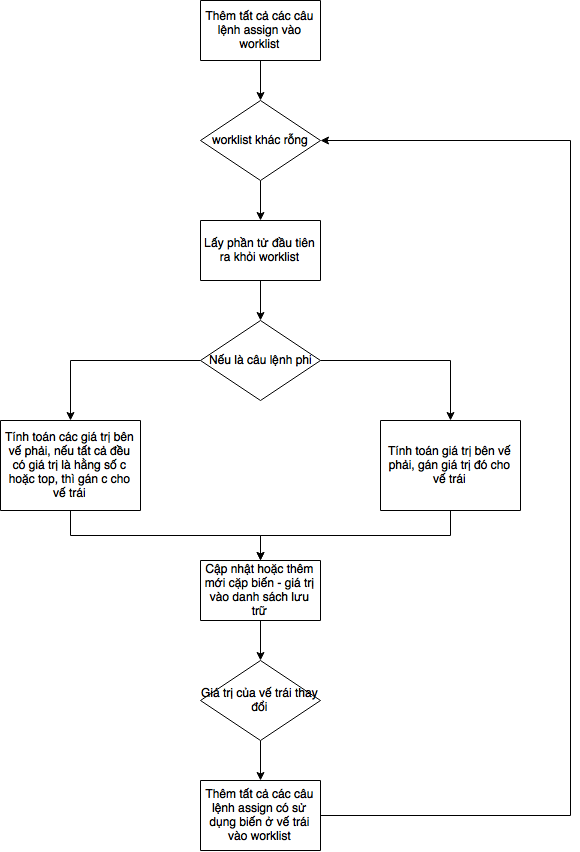
\includegraphics[scale=0.75]{image/constantPropagationAlgo}
	\caption{Giải thuật Constant propagation đã được điều chỉnh phù hợp với yêu cầu của trình dịch ngược}
	\label{fig:constantpropagationalgo}
\end{figure}

Để thể hiện giá trị của một biến có thể thuộc ba loại là top, hằng số hoặc bottom, cần tạo ra một class mới để lưu trữ loại giá trị, đồng thời lưu trữ giá trị thực sự nếu biến đó là một hằng số. Class này được đặt tên là ConstantVariable và có khai báo được trình bày ở đoạn mã \ref{list:listconstexam5}
\begin{lstlisting}[caption={Đoạn mã thể hiện class ConstantVariable},label={list:listconstexam5}, language=c++]
class ConstantVariable{
	public:
	int type; //1: top, 2: constant, 3: bottom
	Exp* variable;
	ConstantVariable(){
		type = 3;
	}
};
\end{lstlisting}
Như vậy, mục tiêu của giải thuật này là tạo ra được một sơ đồ liên kết giữa một biến SSA và một thực thể ConstantVariable thể hiện giá trị của biến đó. \\

Ngoài ra, để tính toán được giá trị thực sự của một biến, cần phải có một hàm chức năng nhận vào một biểu thức và trả về được giá trị của biểu thức đó. Có rất nhiều cách để hiện thực chức năng này, sau một quá trình xem xét, visitor sẽ được sử dụng cho việc tính toán giá trị của biểu thức. Visitor là một pattern design trong các chương trình lập trình hướng đối tượng, nó được dùng để tách một thuật toán ra khỏi cấu trúc dữ liệu mà thuật toán đó sử dụng. Lợi ích đạt được là người lập trình có thể thêm những chức năng mới cho cấu trúc dữ liệu đó mà không cần thay đổi kiến trúc của nó. Điều này phù hợp với nhu cầu hạn chế tối đa việc thay đổi các mã có sẵn khi hiện thực các giải pháp của luận văn trên một trình dịch ngược nào đó.\\

Để hiện thực pattern design này, cần tạo ra một class visitor và viết hàm visit cho các loại biểu thức. Các hàm visit này chính là nơi tính toán giá trị của biểu thức và trả về chúng. Vì biểu thức ở mức assembly thường được viết rất đơn giản, nên trong class visitor này chỉ cần có một số hàm visit cho các loại biểu thức sao đây:

\begin{itemize}
	\item Const: Là biểu thức hằng số. Hàm visit này chỉ đơn giản trả về giá trị hằng số nếu đây là một hằng số nguyên.
	\item Binary: Là biểu thức có 2 vế. Hàm visit sẽ visit từng vế của biểu thức, và nếu cả hai vế đều là hằng số, thì sẽ thực hiện phép tính cộng trừ nhân chia hai hằng số đó để ra được kết quả cuối cùng.
	\item RefExp: Loại biểu thức này chứa một biểu thức khác, kèm theo câu lệnh khai báo biểu thức đó. Trong giới hạn nhu cầu của bài toán, chỉ những RefExp chứa biểu thức là một biến hoặc một thanh ghi được tính toán tiếp, còn những loại biểu thức kia sẽ mặc định trả về giá trị là bottom. Tên biến hoặc biểu thức sẽ được dò tìm trong bảng lưu trữ dữ liệu hằng số và bảng lưu trữ dữ liệu của câu lệnh \#DEFINE để tìm ra được giá trị thực sự của chúng và trả về.
	\item TypedExp: Loại biểu thức để ép kiểu một biểu thức nào đó thành kiểu mong muốn. Với trường hợp này, giá trị trả về của biểu thức ép kiểu chính là giá trị của biểu thức con bên trong.
\end{itemize}


Như vậy, với phương pháp phân tích này, vấn đề vế phải của phép gán thanh ghi là những biểu thức phức tạp có hai toán hạng đã được giải quyết. Ngoài ra, phân tích này còn nhận biết được các biểu thức có giá trị giống nhau mặc dù hình thức bên ngoài khác nhau. Xem ví dụ các câu lệnh ở đoạn mã \ref{list:listdiffassignacc}. Câu lệnh gán số 1 và số 2 thực chất đều gán cho ACC giá trị vùng nhớ có địa chỉ quy định bởi biến OPTIONS. Nếu thực hiện phân tích Reaching definitions ở giải pháp trước, trình dịch ngược sẽ không thể biết được điều này. Tuy nhiên, ở giai đoạn này, vì trình dịch ngược sẽ tính toán được ở cả hai câu lệnh, ACC đều mang giá trị của vùng nhớ có địa chỉ là 38. Và ở những bước tiếp theo, trình dịch ngược sẽ đối chiếu giá trị 38 với bảng lưu trữ dữ liệu và biết được biến OPTIONS đại diện cho giá trị đó.

\begin{lstlisting}[caption={Một số câu lệnh gán cho ACC có giá trị vế phải bằng nhau},label={list:listdiffassignacc}]
#DEFINE OPTIONS #38
#DEFINE CLAMP #37
...
MOV ACC, OPTIONS
MOV ACC, CLAMP+1
\end{lstlisting}

Phân tích Constant propagation sẽ trả về được giá trị thực sự của một biến, tuy nhiên, thanh ghi ACC là một trường hợp đặc biệt. Khi gặp vế trái của câu lệnh khai báo là thanh ghi ACC, giá trị thực sự không được quan tâm, mà chỉ giá trị của địa chỉ vùng nhớ đang được ACC lưu giữ mới được xét đến. Như vậy, chỉ có các câu lệnh dạng MOV ACC, [biểu thức] sẽ được tính toán còn khi gặp câu lệnh gán có dạng MOV ACC, \#[biểu thức] thì đoạn mã phân tích sẽ xem như giá trị của ACC không phải là hằng số (bottom). Như vậy, với các biến khác, giá trị lưu trong thực thể ConstantExpression tương ứng với biến đó là giá trị thực sự của biến, còn riêng với thanh ghi ACC, giá trị đó được hiểu là giá trị địa chỉ vùng nhớ mà thanh ghi ACC được load vào.
\section{Tìm kiếm mối quan hệ giữa các biến}
\subsection{Chuyển đổi giữa hằng số nguyên - biến byte tương ứng}
\label{sec:transfer}
Trước khi bước vào giai đoạn kiểm tra và ghi nhận mối quan hệ giữa các biến, trình dịch ngược cần phải giải quyết kết quả trả về của phương pháp phân tích Constant propagation ở trên. Như đã trình bày, phương pháp này cho biết chính xác giá trị địa chỉ vùng nhớ được lưu trữ bởi thanh ghi ACC. Tuy nhiên, cần phải chuyển đổi con số này thành một biến byte có giá trị bằng nó vì mục đích cuối cùng vẫn là tìm mối quan hệ giữa các biến byte - biến bit. Có hai giải pháp cho vấn đề này:
\begin{itemize}
	\item Ở bất kỳ vị trí nào cần biết được biến byte đang quy định vùng nhớ lưu bởi ACC, lấy giá trị thực sự của địa chỉ vùng nhớ đó và dò tìm trong bảng lưu trữ dữ liệu các câu lệnh \#DEFINE để tìm ra biến byte tương ứng với giá trị đó.
	\item Tạm thời chấp nhận thay vì tìm kiếm mối quan hệ giữa biến byte - biến bit thì sẽ tìm kiếm mối quan hệ giữa giá trị trực tiếp - biến bit. Giá trị này chính là địa chỉ vùng nhớ mà thanh ghi ACC đang lưu trữ tại thời điểm sử dụng biết bit. Sau khi tìm ra các bộ giá trị - biến bit, thêm vào trình dịch ngược một bước chuyển đổi từ giá trị sang biến byte tương ứng dựa vào các câu lệnh khai báo giá trị biến byte ở chương trình đầu vào.
\end{itemize}

Hai giải pháp trên được mô tả lần lượt ở hình \ref{fig:waytotransfer1} và hình \ref{fig:waytotransfer2}. Qua hai sơ đồ trên, dễ dàng nhận ra giải pháp thứ hai sẽ giúp tiết kiệm thời gian xử lý chương trình hơn, nhờ vào việc chỉ cần truy xuất bảng dữ liệu ở cuối giai đoạn tìm kiếm. Còn giải pháp đầu tiên không hiệu quả do mỗi lần cần kiểm tra giá trị của thanh ghi ACC lại phải tìm kiếm dữ liệu. Như vậy, giải pháp thứ hai sẽ được áp dụng.
\begin{figure}
	\centering
	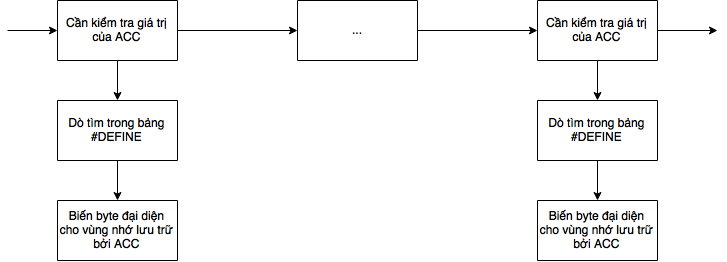
\includegraphics[width=0.7\linewidth]{image/wayToTransfer1}
	\caption{Giải pháp chuyển đổi giá trị - biến byte số 1}
	\label{fig:waytotransfer1}
\end{figure}
\begin{figure}
	\centering
	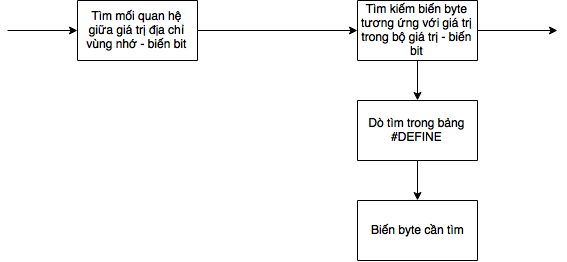
\includegraphics[width=0.7\linewidth]{image/wayToTransfer2}
	\caption{Giải pháp chuyển đổi giá trị - biến byte số 2}
	\label{fig:waytotransfer2}
\end{figure}
\subsection{Kiểm tra và ghi nhận mối quan hệ giữa các giá trị - biến bit}
 Nếu như ở giải pháp Kiểm tra kiểu, mối quan hệ biến byte - biến bit đã được cho trước và trình dịch ngược chỉ cần kiểm tra lại thì ở giải pháp này, vì không có thông tin từ phần chú thích của người lập trình, trình dịch ngược phải tự tìm kiếm các mối quan hệ giữa các giá trị địa chỉ vùng nhớ và biến bit, kiểm tra tính hợp lệ của chúng và ghi nhận vào danh sách dữ liệu. Các bước này được thể hiện ở hình \ref{fig:stepunionmaking}. Giai đoạn kiểm tra tính hợp lệ nhằm đảm bảo là các bộ biến được sử dụng theo đúng nguyên tắc đã giới thiệu ở chương đầu.
\begin{figure}[h]
	\centering
	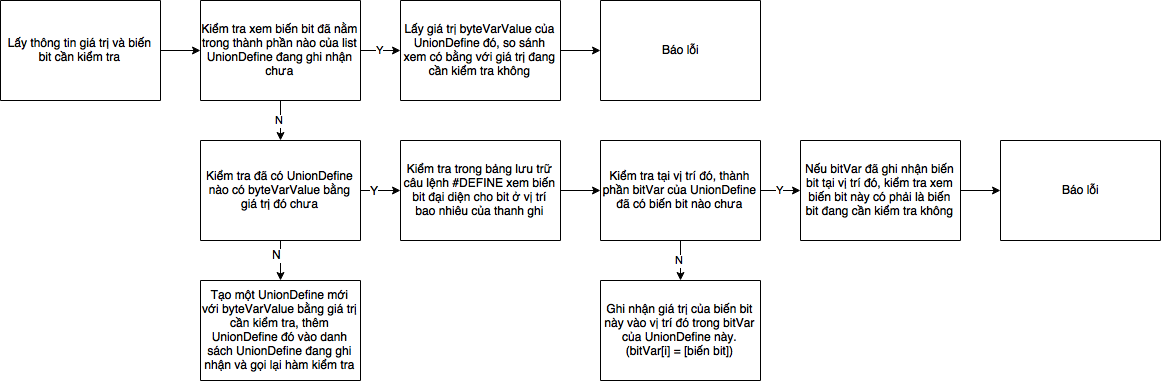
\includegraphics[width=0.7\linewidth]{image/stepUnionMaking}
	\caption{Các bước kiểm tra và ghi nhận dữ liệu vào danh sách UnionDefine}
	\label{fig:stepunionmaking}
\end{figure}

Như đã trình bày ở phần \ref{sec:transfer}, thay vì tìm kiếm các bộ biến byte - biến bit thì ở giai đoạn này sẽ tìm kiếm các bộ giá trị địa chỉ vùng nhớ - biến bit, vì vậy, cấu trúc lưu trữ dữ liệu tìm thấy được cũng phải được chỉnh sửa để ghi nhận mối quan hệ mới này. Cấu trúc UnionDefine được giới thiệu ở chương trước vẫn tiếp tục được sử dụng, tuy nhiên, được mở rộng thêm một trường dữ liệu mới là byteVarValue để ghi nhận giá trị địa chỉ vùng nhớ của bộ biến. Đoạn mã mới được trình bày bên dưới.

\begin{lstlisting}[caption={Đoạn mã mới của class UnionDefine},label={list:listnewuniondefine},language=c++]
	class UnionDefine{
	public:
	char* byteVar;
	map<int, char*>* bitVar;
	int byteVarValue;
 };
\end{lstlisting}
Sau khi đã quét hết các câu lệnh ở các procedure, trước khi chuyển đổi các UnionDefine thành các khai báo ở ngôn ngữ C và thêm vào danh sách các biến toàn cục của program như giải pháp trước, cần phải thêm vào một bước chuyển đổi từ giá trị thành biến byte đại diện cho giá trị đó. Điều này có thể được thực hiện bằng cách chạy vòng lặp qua bảng lưu trữ các câu lệnh \#DEFINE đã được thiết lập từ quá trình parse mã đầu vào. Nếu như có một giá trị nào đó chưa được khai báo ở câu lệnh \#DEFINE, một biến byte mới sẽ được sinh ra để đại diện cho giá trị ấy. Mẫu tên biến byte sẽ là LOCATION\_[giá trị của biến byte], ví dụ như LOCATION\_38.

Như vậy, giải pháp này đã giải quyết được các vấn đề đặt ra của luận văn. 
	\chapter{Kiểm tra kết quả}

Bất kỳ một sản phẩm nào đều cần phải được kiểm tra trước khi công bố, luận văn này cũng không phải là một ngoại lệ. Để đảm bảo chất lượng được đánh giá một các khách quan nhất, một hệ thống testcase với các loại tình huống được phân bổ một cách khoa học sẽ được đưa ra, chỉnh sửa cho phù hợp với 2 bài toán của luận văn là Kiểm tra kiểu và Suy luận kiểu và chạy thử để đưa ra kết quả. Tuy nhiên, để chạy được các giải pháp của luận văn, cần chọn một trình dịch ngược sẵn có và chỉnh sửa, hiện thực giải pháp trên đó. Trình dịch ngược được chọn là Boomerang như đã trình bày ở phần \ref{sec:whyboom}. Phần đầu của chương này sẽ trình bày các thiết lập cần thiết trên Boomerang để hiện thực giải pháp cho kiến trúc máy 8051 như phần giới hạn của chương trình. Phần tiếp theo đề ra phương pháp kiểm thử bao gồm cách lập testcase và kết quả chạy thử testcase trên các giải pháp.

\section{Thiết lập Boomerang}

\label{sec:boomchange}
Ở phần \ref{sec:whyboom}, một bảng đánh giá các trình dịch ngược hiện tại đã được đưa ra để lựa chọn trình dịch ngược phù hợp nhất để hiện thực giải pháp và Boomerang đã được chọn vì có số điểm ở các tiêu chí cao nhất. Tuy nhiên, để hiện thực các thuật toán của luận văn, cần có các chỉnh sửa sau:
\begin{itemize}
	\item Xử lý để Boomerang giữ được tên biến được người dùng tự khai báo. Vì bản thân Boomerang là một trình dịch ngược từ mã máy, nên nó chỉ xử lý dữ liệu dưới dạng thanh ghi, các thanh ghi này phải được định nghĩa trước trong file đặc tả của từng kiến trúc máy.
	\item Chỉnh sửa giai đoạn sinh mã của Boomerang. Các giải pháp đưa ra trong luận văn đều có kết quả cuối cùng là một danh sách các UnionDefine tương ứng với những union tìm thấy được. Để đưa các UnionDefine này thành các cấu trúc union ở mã đầu ra, cần phải có một số thay đổi ở phần sinh mã của Boomerang
\end{itemize}
Các thay đổi này sẽ	 lần lượt được trình bày ở các phần dưới.

\subsection{Thay đổi cơ chế quản lý tên dữ liệu của Boomerang}

Vì ở mức độ mã máy, dữ liệu chỉ được lưu ở các thanh ghi cố định hoặc vùng nhớ được truy xuất bằng địa chỉ nên Boomerang không có cơ chế xử lý các biến được người dùng tạo ra ở mã assembly. Tuy nhiên, Boomerang vẫn có cơ chế để giữa được tên các thanh ghi đó ở đoạn mã đầu ra, nên cần tìm hiểu về cơ chế này và chỉnh sửa để nó linh hoạt chấp nhận tất cả các tên biến khác chứ không chỉ riêng tên thanh ghi.

\subsubsection{Phương thức lưu trữ tên thanh ghi của Boomerang}
Khi chuyển đổi từ mã assembly sang mã trung gian, Boomerang sẽ dùng một class con của \textit{Expr} để biểu diễn thanh ghi. Cụ thể là class \textit{Location}, và gọi phương thức static của class \textit{Location} là \textit{Location::regOf(int num)}, phương thức này cần được truyền vào một con số đại diện cho thanh ghi. Cặp số - tên thanh ghi này được lưu vào một từ điển, để sau này khi thực hiện phân tích xong thì sẽ chuyển lại từ thanh ghi thành biến cục bộ.

Trong phần giải mã từ mã assembly sang mã trung gian, có một hàm để map giữa tên thanh ghi và con số đại diện cho nó, đó là hàm \textit{map\_sfr(string name)} được thể hiện ở đoạn mã \ref{list:listmapsfr}.
\begin{lstlisting}[caption={Một số phần mã trong hàm map\_sfr},label={list:listmapsfr},language=c++]
if (name == "R0") return 0;
else if (name == "R1") return 1;
else if (name == "R2") return 2;
...
else return -1;

\end{lstlisting}

Sau khi trải qua các quá trình phân tích và đến giai đoạn in ra mã đầu ra, trình dịch ngược sẽ gọi hàm \textit{getRegName} trong class \textit{FrontEnd} để trả lại tên ban đầu của thanh ghi. Hàm này được trình bày ở đoạn mã \ref{list:listgetregname}. Trong hàm \textit{getRegName}, Boomerang sẽ lấy từ điển tên thanh ghi - số đại diện được quy định sẵn trong đặc tả của các kiến trúc máy, tìm tên thanh ghi tương ứng với con số đó và trả về.
\begin{lstlisting}[caption={Phần mã trong hàm getRegName},label={list:listgetregname},language=c++]
std::map<std::string, int, std::less<std::string>>::
																				iterator it;
for (it = decoder->getRTLDict().RegMap.begin();	 it != 										
	decoder->getRTLDict().RegMap.end(); it++)
	if ((*it).second == idx) 
		return (*it).first.c_str();
return NULL;
\end{lstlisting}


Như vậy, có thể thấy với các tên biến không được quy định trước, hàm \textit{map\_sfr} sẽ trả về giá trị \textbf{-1}, và vì giá trị \textbf{-1} sẽ không có trong từ điển của kiến trúc máy, nên hàm \textit{getRegName} sẽ trả về \textbf{NULL}, dẫn đến trình dịch ngược sẽ bị lỗi runtime và dừng ngay lập tức.\\

%lấy mã Boomerang ban đầu về, hiện kết quả khi sử dụng biến đầu vào

\subsubsection{Chỉnh sửa phương thức trên để chấp nhận tên biến tự khai báo}
Vì số lượng tên biến là rất nhiều, nên giải pháp thêm mới các tên biến vào từ điển được quy định sẵn là không khả thi, mà phải có cách để trình dịch ngược linh động hơn, chấp nhận bất kỳ các tên nào được sử dụng trong mã assembly. Giải pháp đưa ra là ngoài việc sử dụng từ điển thanh ghi được quy định sẵn, một bảng tên biến sẽ được lập thêm, thành phần bao gồm các cặp tên biến - số đại diện. Trong giai đoạn giải mã, khi hàm \textit{map\_sfr} được gọi, nếu tên truyền vào nằm trong các thanh ghi đã quy định sẵn, thay vì trả về giá trị \textbf{-1} thì ta sẽ tạo ra một giá trị random và đưa chúng vào bảng tên biến ở trên. Ngoài ra, còn có một đoạn mã kiểm tra biến được sử dụng đã được khai báo chưa (ngoại trừ một số biến đặc biệt được tự sinh). Hàm \textit{map\_sfr} nâng cấp được trình bày trong đoạn mã \ref{list:listmapsfrnew}.\\
\begin{lstlisting}[caption={Phần mã mới được bổ sung trong hàm map\_sfr},label={list:listmapsfrnew},language=c++]
bool isDefined = false;
map<char*, AssemblyArgument*>::iterator it;
for (it = replacement.begin(); it!=replacement.end()
		; it++){
	if(strcmp((*it).first, name.c_str()) == 0 ){
		isDefined = true;
		break;
	}
}
if (isDefined || name.find("specbits") != string::npos ){
	if (symbolTable->find(name) 
		== symbolTable->end()){
		bool existed = false;
		int num;
		do{
			num = std::rand()%200+31;
			map<string, int>::iterator it;
			for (it = symbolTable->begin(); it!=symbolTable->end()
				; it++){
				bool cond1 = (*it).second == num;
				bool cond2 = (byteVar != -1 && byteVar>=num);
				bool cond3 = (bit != -1 && bit>=num);
				if (cond1 || cond2 || cond3){
					existed = true;
					continue;
				} else {
					existed = false;
				}	
			}
		} while (existed); 
		(*symbolTable)[name] = num;
		if (name.find("specbits") != string::npos){
			std::cout<<"Name: "<<name<<", "<<num<<endl;
		}	
		return num;
	} else {
		return symbolTable->find(name)->second;
	}
}
else {
	std::cout<<"ERROR: "<<name<<" HAS NOT BEEN DEFINED YET"
			<<endl;
	exit(1);
}
\end{lstlisting}
Tương ứng với sự thay đổi ở hàm \textit{map\_sfr},  ở hàm \textit{getRegName}, ngoài việc dò trong từ điển quy định trước, cần phải bổ sung thêm một đoạn mã để dò trong bảng tên biến. Phần bổ sung này được thể hiện ở đoạn mã \ref{list:listgetregnamenew}.
\begin{lstlisting}[caption={Phần mã mới được bổ sung trong hàm getRegName},label={list:listgetregnamenew},language=c++]
std::map<string,int>::iterator symIt;
for (symIt = decoder->getSymbolTable().begin(); symIt != 
	decoder->getSymbolTable().end(); symIt++){
	if ((*symIt).second == idx){
		return (*symIt).first.c_str();
	}
}
\end{lstlisting}
Như vậy, vấn đề giữ nguyên tên biến được giải quyết mà không ảnh hưởng nhiều tới trình dịch ngược.
%đoạn mã đầu vào assembly và mã đầu ra giữ nguyên được tên biến

\subsection{Thêm trường hợp cấu trúc union vào đoạn sinh mã của Boomerang}

Từ dữ liệu là danh sách các thực thể UnionDefine được rút trích thông qua các giải thuật của luận văn, trình dịch ngược cần phải đưa ra các union tương ứng. Hình \ref{fig:uniondefinemapping} thể hiện việc chuyển đổi của class UnionDefine cho kiến trúc máy 8051 sang cấu trúc union. Các union này được thêm vào danh sách biến toàn cục (global) của chương trình vì chúng có tác dụng trên toàn chương trình chứ không riêng một hàm nào.

\begin{figure}[h!]
\centering
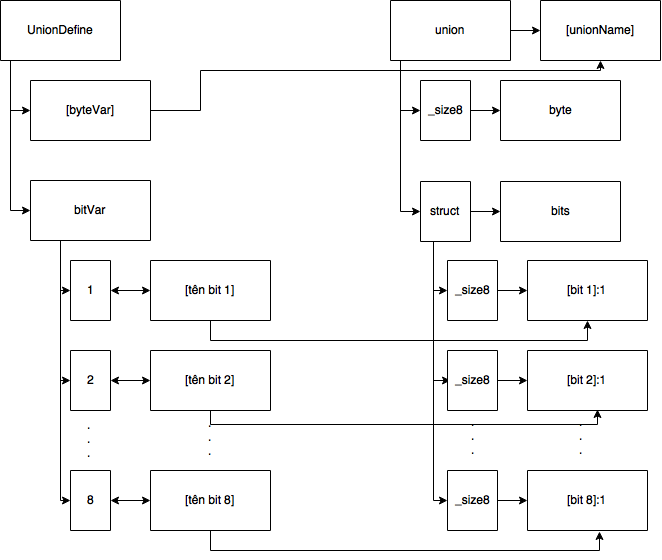
\includegraphics[width=\linewidth]{image/unionDefineMapping}
\caption{Hình minh hoạ việc chuyển đổi từ class UnionDefine cho mã 8051 sang cấu trúc union ở mã đầu ra}
\label{fig:uniondefinemapping}
\end{figure}

Sau khi sinh ra các union như trên, một số thay thế cần được thực hiện trên đoạn mã đầu ra. Cụ thể như sau:
\begin{itemize}
\item Thay thế các biểu thức thể hiện các thành phần của union dưới dạng thanh ghi độc lập thành một biểu thức truy xuất đến union đó. Vì ở giai đoạn giải mã, chưa có thông tin nào về các kiểu union, nên trình dịch ngược sẽ xem tất cả các biến là những đối tượng dữ liệu độc lập với nhau. Sau khi đã trải qua các quá trình phân tích và sinh ra các union, ta cần thay thế để thể hiện rõ mối liên hệ giữa các thành phần của những union đó. Ví dụ như ở đoạn mã \ref{list:listbeforereplacebitvar}, thành phần \textit{TESTSUPS} vẫn đang được xem như là một biến độc lập ở mã đầu ra, và cần phải thay thế nó bằng một truy xuất tới union chứa thành phần \textit{TESTSUPS}, trong trường hợp này là \textit{OPTIONS}. Kết quả của bước thay thế này được thể hiện ở đoạn mã \ref{list:listafterreplacebitvar}.
\begin{lstlisting}[caption={Mã đầu ra trước khi thực hiện các bước thay thế},label={list:listbeforereplacebitvar}, language = c]
a = *OPTIONS;
TESTSUPS = 1;
if (specbits1 == 1){
	...
}
return a;
\end{lstlisting}

\begin{lstlisting}[caption={Mã đầu ra sau khi thực hiện bước thay thế thành phần của union},label={list:listafterreplacebitvar}, language = c]
a = *OPTIONS;
OPTIONS.bits.TESTSUPS = 1;
if (specbits1 == 1){
	...
}
return a;
\end{lstlisting}
\item Thay thế các biểu thức truy xuất trực tiếp một phần của thanh ghi trung gian thành biểu thức truy xuất đến thành phần tương ứng trong kiểu union của thanh ghi đó. Vì một số lý do, có đôi khi lập trình viên không sử dụng tên biến mà dùng biểu thức truy xuất trực tiếp đến một thành phần của thanh ghi trung gian. Ví dụ như trong 8051, người lập trình có thể dùng biểu thức \textit{ACC.1 }để truy xuất tới bit đầu tiên của thanh ghi \textit{ACC}. Với trường hợp này, vì đã có dữ liệu về kiểu union mà thanh ghi trung gian đang mang, các biểu thức dạng này sẽ được thay thế bằng biểu thức truy xuất đến union để đoạn mã đầu ra thống nhất hơn, và có thể tiến hành bước thay thế thanh ghi trung gian được trình bày bên dưới. Lưu ý: trong giai đoạn giải mã, các biểu thức truy xuất trực tiếp này sẽ được thể hiện dưới dạng đặc biệt để dễ dàng nhận biết sau này. Ví dụ như với mã 8051, khi gặp biểu thức \textit{ACC.x}, trình giải mã sẽ chuyển chúng về một thanh ghi đặc biệt có tên là \textit{specbitsx}, với \textit{x} là số thứ tự của bit muốn truy xuất như ở đoạn mã \ref{list:listbeforereplacebitvar}. Tiếp tục ví dụ nêu trên, các truy xuất trực tiếp tới bit của thanh ghi \textit{ACC} cũng được thay thế bằng các biểu thức truy thành phần của union tương ứng. Kết quả là đoạn mã \ref{list:listafterreplacebit}, biến đặc biệt \textit{specbits1} đã được thay thế thành biểu thức \textit{OPTIONS.bits.bit1}.

\begin{lstlisting}[caption={Mã đầu ra sau khi thực hiện bước thay thế truy xuất trực tiếp đến một phần của thanh ghi trung gian},label={list:listafterreplacebit}, language = c]
a = *OPTIONS;
OPTIONS.bits.TESTSUPS = 1;
if (OPTIONS.bits.bit1 == 1){
	...
}
return a;
\end{lstlisting}
\item Thay thế các vị trí sử dụng thanh ghi trung gian bằng union tương ứng. Khi lập trình ở dạng mã assembly, lập trình viên không được phép xử lý các vùng nhớ trực tiếp mà phải thông qua thanh ghi trung gian, tuy nhiên, khi đã chuyển đổi về dạng ngôn ngữ cấp cao, có thể sử dụng trực tiếp tên union trong các câu lệnh mà không cần trung gian qua thanh ghi nữa. Điều này giúp mã đầu ra ngắn gọn, dễ hiểu và trong sáng hơn. Đoạn mã \ref{list:listafterreplaceacc} là kết quả sau khi thực hiện bước thay thế này. Dễ dàng thấy đoạn mã đã gọn hơn rất nhiều do loại bỏ được câu lệnh gán cho biến \textit{a}, và thay thế biến \textit{a} ở câu lệnh return thành truy xuất \textit{OPTIONS.byte}. Vì thực chất \textit{a} đang mang kiểu union \textit{OPTIONS}, nên đoạn mã này hoàn toàn tương đương với đoạn mã ở \ref{list:listafterreplacebit}.

\begin{lstlisting}[caption={Mã đầu ra sau khi thực hiện bước thay thế thanh ghi trung gian},label={list:listafterreplaceacc}, language = c]
OPTIONS.bits.TESTSUPS = 1;
if (OPTIONS.bits.bit1 == 1){
	...
}
return OPTIONS.byte;
\end{lstlisting}
\end{itemize}

Có thể thấy, sau khi thực hiện các bước thay thế mã ở trên, đoạn mã cuối cùng ở hình \ref{list:listafterreplaceacc} đã gọn và dễ đọc hơn rất nhiều so với đoạn mã ban đầu \ref{list:listbeforereplacebitvar}.
\section{Kiểm tra kết quả luận văn trên Boomerang}

\subsection{Hệ thống testcase}
Có các tiêu chí phân loại testcase như sau:
\begin{itemize}
	\item Loại biểu thức được gán vào thanh ghi trung gian (tiêu chí I)
	\item Cách truy xuất một thành phần của thanh ghi (tiêu chí II)
	\item Có vi phạm nguyên tắc sử dụng kiểu union hay không (tiêu chí III)
\end{itemize}
Với mỗi tiêu chí, ta sẽ có các trường hợp sau đây:

Tiêu chí I:
\begin{enumerate}
	\item Một hằng số (I.1)
	\item Giá trị ở một vùng nhớ có địa chỉ là một biến (I.2)
	\item Giá trị ở một vùng nhớ có địa chỉ là một hằng số (I.3)
	\item Giá trị ở một vùng nhớ có địa chỉ là một thanh ghi (I.4)
	\item Giá trị ở một vùng nhớ có địa chỉ là một biểu thức 2 vế. Mỗi vế có thể là một biến byte, một thanh ghi, hoặc một hằng số (I.5)
\end{enumerate}

Tiêu chí II:
\begin{enumerate}
	\item Truy xuất dựa vào một biến đại diện. (II.1)
	\item Truy xuất bằng cấu trúc truy xuất trực tiếp một phần nhỏ hơn của thanh ghi. Ví dụ: \textit{ACC.5} trong mã 8051. (II.2)
\end{enumerate}

Tiêu chí III:
\begin{enumerate}
	\item Không vi phạm nguyên tắc sử dụng kiểu union. (III.1)
	\item Một thành phần của union này được sử dụng khi thanh ghi trung gian đang có kiểu là một union khác. Như ví dụ ở đoạn mã \ref{list:invalid1}, thành phần \textit{TESTUPS} được xác định thuộc union \textit{OPTIONS} thông qua 2 câu lệnh 1 và 2, nhưng sau đó lại được truy xuất ở câu lệnh số 4 khi mà thanh ghi trung gian \textit{ACC} đang mang kiểu union \textit{OPTIONS2}. (III.2)
	\begin{lstlisting}[caption={Đoạn mã có một biến bit thuộc nhiều bộ biến khác nhau},label={list:invalid1}]
	MOV A, OPTIONS ;1
	SETB TESTSUPS ;2
	...
	MOV A, OPTIONS2 ;3
	JB TESTSUPS, BB ;4
	\end{lstlisting}
	\item Tại một thời điểm sử dụng thành phần của một union, thanh ghi trung gian có thể mang nhiều kiểu union khác. Xem ví dụ ở đoạn mã \ref{list:invalid2}, ở câu lệnh cuối cùng, biến \textit{a} có thể mang kiểu union \textit{OPTIONS} hoặc \textit{OPTIONS2}, như vậy không thể xác định được \textit{TESTSDOWNS} thuộc union nào. (III.3)
	\begin{lstlisting}[caption={Đoạn mã ACC có thể mang nhiều giá trị vùng nhớ khác nhau},label={list:invalid2}, language=c++]
	if (TESTSUPS == 1)
		a = *OPTIONS;
	else
		a = *OPTIONS2;
	TESTSDOWNS = 0;
	\end{lstlisting}
	\item Ghi nhận được có hai thành phần cùng thuộc một union và cùng truy xuất đến một vị trí của union đó. Như ở đoạn mã \ref{list:invalid3}, biến \textit{TESTSUPS} và \textit{TESTSDOWNS} đều được sử dụng để truy xuất tới bit đầu tiên của union \textit{OPTIONS}. (III.4)
	\begin{lstlisting}[caption={Đoạn mã có 2 thành phần union cùng truy xuất đến một vị trí vùng nhớ của union đó},label={list:invalid3}]
	...
	#DEFINE TESTSUPS, ACC.1
	#DEFINE TESTSDOWNS, ACC.1
	...
	MOV A, OPTIONS
	SETB TESTSUPS
	...
	MOV A, OPTIONS
	CLR TESTSDOWNS
	\end{lstlisting}
\end{enumerate}

Kết hợp các tiêu chí trên, loại bỏ đi một số trường hợp không thể xảy ra, có tổng cộng 18 trường hợp cần kiểm thử. Hầu hết mỗi trường hợp sẽ có một testcase đại diện, nhưng với một số trường hợp phức tạp sẽ có nhiều testcase hơn. Bảng 5.1 thể hiện việc phân bổ testcase theo các trường hợp của các tiêu chí.
\begin{table}[h!]
	\centering
	\begin{tabular}{ |p{0.7cm}| p{2cm}| p{2cm}| p{2cm}| p{5cm}|}
		\hline
		
		STT & Tiêu chí I & Tiêu chí II & Tiêu chí III & Mã testcase\\
		\hline
		1 & 1 & 1 & 1 &TC001\\
		\hline
		2 & 1 & 2 & 1 &TC002\\
		\hline
		3 & 2 & 1 & 1 &TC003\\
		\hline
		4 & 2 & 2 & 1 &TC004\\
		\hline
		5 & 3 & 1 & 1 &TC005\\
		\hline
		6 & 3 & 2 & 1 &TC006\\
		\hline
		7 & 4 & 1 & 1 &TC007, TC019, TC024\\
		\hline
		8 & 4 & 2 & 1 &TC008\\
		\hline
		9 & 5 & 1 & 1 &TC009\\
		\hline
		10 & 5 & 2 & 1 &TC010, TC020\\
		\hline
		11 & 2-3& 1 & 2 &TC011\\
		\hline
		12 & 4-5 & 1 & 2 &TC012\\
		\hline
		13 & 2-3 & 1 & 3 &TC013, TC023\\
		\hline
		14 & 2-3 & 2 & 3 &TC014\\
		\hline
		15 & 4-5 & 1 & 3 &TC015, TC021, TC022\\
		\hline
		16 & 4-5 & 2 & 3 &TC016\\
		\hline
		17 & 2-3 & 1 & 4 &TC017\\
		\hline
		18 & 4-5 & 1 & 4 &TC018\\
		\hline
	\end{tabular}
	
	
	\label{table:table2}
	\caption{Bảng phân bổ các testcase theo từng trường hợp của các tiêu chí}
\end{table}
\subsection{Kết quả chạy thử}

Tuỳ thuộc vào bài toán cần kiểm tra kết quả là gì, các testcase sẽ được điều chỉnh cho phù hợp. Với bài toán Kiểm tra kiểu, phần khai báo của testcase phải cung cấp thông tin về các union theo mẫu quy định, còn bài toán Suy luận kiểu thì không cần. Tuy nhiên nội dung của của các testcase được giữ nguyên để đảm bảo kết quả chạy ra của hai bài toán là như nhau. Kết quả chạy thử các testcase trên từng bài toán được thể hiện ở bảng 5.2

\begin{table}[h!]
	\centering
	\begin{tabular}{ |p{0.7cm}| p{3cm}| p{5cm}| p{5cm}|}
		\hline
		
		STT & Tiêu chí & Bài toán Kiểm tra kiểu & Bài toán Suy luận kiểu\\
		\hline
		1 & Số testcase đúng & 15/24 & 24/24\\
		\hline
		2 & Các testcase bị sai &TC009, TC010, TC012, TC015, TC016, TC018, TC020, TC021, TC022 &\\
		\hline
		3 & Nguyên nhân bị sai & Do phương pháp phân tích dữ liệu được sử dụng không xử lý được hết các trường hợp biểu thức quy định địa chỉ vùng nhớ gán cho thanh ghi trung gian, nên những testcase mà biểu thức này có hai toán hạng sẽ bị sai & \\
		\hline
	\end{tabular}
	
	
	\label{table:table3}
	\caption{Bảng kết quả chạy thử testcase cho hai bài toán}
\end{table}
Như vậy, có thể thấy với bài toán Kiểm tra kiểu, có nhiều testcase cho ra kết quả sai, còn bài toán Suy luận kiểu thì tất cả các trường hợp đều chính xác. Điều này đã được dự báo trước vì kỹ thuật phân tích sử dụng trong bài toán Kiểm tra kiểu còn nhiều hạn chế.\\


	\chapter{Kết luận}

Chương này sẽ tổng kết lại các kết quả đã đạt được của luận văn và đưa ra hướng phát triển trong tương lai.

\section{Kết quả đạt được}

Nhìn chung, luận văn đã hoàn thành mục tiêu đề ra ban đầu, giải quyết được bài toán về kiểu dữ liệu bit và câu lệnh xử lý bit trong mã assembly của 8051. Ngoài ra, luận văn đã chứng minh được tính thực tiễn của đề tài, khả năng áp dụng vào thực tế của các doanh nghiệp có nhu cầu dịch ngược. Cuối cùng, luận văn cũng đưa ra một phương pháp lập testcase và kiểm thử khoa học, đảm bảo đưa ra được các trường hợp có thể xảy ra ngoài thực tế và đặc biệt có một testcase là một đoạn mã thật của doanh nghiệp. Kết quả kiểm thử trên bộ testcase dành cho phương pháp Suy luận kiểu là chấp nhận được.

\section{Hướng phát triển trong tương lai}

Các hướng phát triển trong tương lai của trình dịch ngược gồm có:

\begin{itemize}
	\item Tiếp tục mở rộng khả năng dịch ngược cho nhiều máy khác nhau.
	\item Phân tích và sửa lỗi sai của giải thuật phân tích dòng dữ liệu.
	\item Cải tiến chức năng nhận dạng kiểu của Boomerang.
	\item Áp dụng các giải thuật nhận dạng union được trình bày trong luận văn này cho các kiến trúc máy có tính chất tương tự 8051.
\end{itemize}

	
	\newpage
	\nocite{*}
	\printbibliography

\end{document}